\documentclass[12pt]{article}
\usepackage{fullpage,marginnote,caption}

\usepackage{amsfonts}
\usepackage{amsmath}
\usepackage{amssymb}
\usepackage{amsthm}
\usepackage{graphicx}

\usepackage{framed}
\usepackage{hyperref}

\setlength{\parskip}{\baselineskip}%
\setlength{\parindent}{0pt}%

\title{EE 127/227A Study Guide / Tips and Tricks}
\author{Joshua Achiam}




\begin{document}
%
% Definitions and macros
%

%\setlength{\marginparwidth}{1.2in}
%\let\oldmarginpar\marginpar
%\renewcommand\marginpar[1]{\-\oldmarginpar[\raggedleft\footnotesize #1]%
%{\raggedright\footnotesize #1}}

%\renewcommand{\indexspace}{\rule{0cm}{.4cm}}
%% end example/remark
%\newcommand{\eex}{\ifmmode\sq\else{\unskip\nobreak\hfil
%  \penalty50\hskip1em\null\nobreak\hfil$\Diamond$
%  \parfillskip=0pt\finalhyphendemerits=0\endgraf}\fi{}}
%\newcommand{\erem}{\ifmmode\sq\else{\unskip\nobreak\hfil
%  \penalty50\hskip1em\null\nobreak\hfil$\star$
%  \parfillskip=0pt\finalhyphendemerits=0\endgraf}\fi{}}
%\newcommand{\eobs}{\ifmmode\sq\else{\unskip\nobreak\hfil
%  \penalty50\hskip1em\null\nobreak\hfil$\vartriangleleft$
%  \parfillskip=0pt\finalhyphendemerits=0\endgraf}\fi{}}


% VET - characters - lowercase
\newcommand{\avet}{{\mathbf  a}}
\newcommand{\bvet}{{\mathbf  b}}
\newcommand{\cvet}{{\mathbf  c}}
\newcommand{\dvet}{{\mathbf  d}}
\newcommand{\evet}{{\mathbf  e}}
\newcommand{\fvet}{{\mathbf  f}}
\newcommand{\gvet}{{\mathbf  g}}
\newcommand{\hvet}{{\mathbf  h}}
\newcommand{\ivet}{{\mathbf  i}}
\newcommand{\jvet}{{\mathbf  j}}
\newcommand{\kvet}{{\mathbf  k}}
\newcommand{\lvet}{{\mathbf  l}}
\newcommand{\mvet}{{\mathbf  m}}
\newcommand{\nvet}{{\mathbf  n}}
\newcommand{\ovet}{{\mathbf  o}}
\newcommand{\pvet}{{\mathbf  p}}
\newcommand{\qvet}{{\mathbf  q}}
\newcommand{\rvet}{{\mathbf  r}}
\newcommand{\svet}{{\mathbf  s}}
\newcommand{\tvet}{{\mathbf  t}}
\newcommand{\uvet}{{\mathbf  u}}
\newcommand{\vvet}{{\mathbf  v}}
\newcommand{\xvet}{{\mathbf  x}}
\newcommand{\yvet}{{\mathbf  y}}
\newcommand{\zvet}{{\mathbf  z}}
\newcommand{\wvet}{{\mathbf  w}}

% VET - characters - uppercase
\newcommand{\Avet}{{\mathbf  A}}
\newcommand{\Bvet}{{\mathbf  B}}
\newcommand{\Cvet}{{\mathbf  C}}
\newcommand{\Dvet}{{\mathbf  D}}
\newcommand{\Evet}{{\mathbf  E}}
\newcommand{\Fvet}{{\mathbf  F}}
\newcommand{\Gvet}{{\mathbf  G}}
\newcommand{\Hvet}{{\mathbf  H}}
\newcommand{\Ivet}{{\mathbf  I}}
\newcommand{\Jvet}{{\mathbf  J}}
\newcommand{\Kvet}{{\mathbf  K}}
\newcommand{\Lvet}{{\mathbf  L}}
\newcommand{\Mvet}{{\mathbf  M}}
\newcommand{\Nvet}{{\mathbf  N}}
\newcommand{\Ovet}{{\mathbf  O}}
\newcommand{\Pvet}{{\mathbf  P}}
\newcommand{\Qvet}{{\mathbf  Q}}
\newcommand{\Rvet}{{\mathbf  R}}
\newcommand{\Svet}{{\mathbf  S}}
\newcommand{\Tvet}{{\mathbf  T}}
\newcommand{\Uvet}{{\mathbf  U}}
\newcommand{\Xvet}{{\mathbf  X}}
\newcommand{\Yvet}{{\mathbf  Y}}
\newcommand{\Vvet}{{\mathbf  V}}
\newcommand{\Wvet}{{\mathbf  W}}
\newcommand{\Zvet}{{\mathbf  Z}}

\newcommand{\Deltavet}{\mathbf  \Delta}
\newcommand{\Lambdavet}{{\mathbf  \Lambda}}
\newcommand{\Sigmavet}{\mathbf  \Sigma}
\newcommand{\Thetavet}{{\mathbf  \Theta}}

% Special characters:
\newcommand{\s}{ {\sigma} }

\newcommand{\e}{{\mathrm e}}
\newcommand{\jm}{{\mathrm j}}
\newcommand{\E}{{\mathrm E}}
\newcommand{\Ex}{{\mathbb E}}
\renewcommand{\d}{{\mathrm d}}
\newcommand{\dt}{{\mathrm d}t}
\newcommand{\X}{ {\mathcal X} }
\newcommand{\Y}{ {\mathcal Y} }
\newcommand{\Z}{ {\mathcal Z} }



\newcommand{\calA}{{\mathcal A}}
\newcommand{\calB}{{\mathcal B}}
\newcommand{\calC}{{\mathcal C}}
\newcommand{\calD}{{\mathcal D}}
\newcommand{\calE}{{\mathcal E}}
\newcommand{\calF}{{\mathcal F}}
\newcommand{\calG}{{\mathcal G}}
\newcommand{\calH}{{\mathcal H}}
\newcommand{\calI}{{\mathcal I}}
\newcommand{\calJ}{{\mathcal J}}
\newcommand{\calK}{{\mathcal K}}
\newcommand{\calL}{{\mathcal L}}
\newcommand{\calM}{{\mathcal M}}
\newcommand{\calN}{{\mathcal N}}
\newcommand{\calO}{{\mathcal O}}
\newcommand{\calP}{{\mathcal P}}
\newcommand{\calQ}{{\mathcal Q}}
\newcommand{\calR}{{\mathcal R}}
\newcommand{\calS}{{\mathcal S}}
\newcommand{\calT}{{\mathcal T}}
\newcommand{\calU}{{\mathcal U}}
\newcommand{\calV}{{\mathcal V}}
\newcommand{\calX}{{\mathcal X}}
\newcommand{\calY}{{\mathcal Y}}
\newcommand{\calW}{{\mathcal W}}
\newcommand{\calZ}{{\mathcal Z}}
\newcommand{\qtil}{{\tilde{q}}}
\newcommand{\td}{{\tilde{\delta}}}

\newcommand{\vect}[1]{ {\mbox{\rm vec}(#1)} }

% Macro comandi:

\newcommand{\Atil}{\tilde{A}}
\newcommand{\Zhat}{\hat{Z}}
\newcommand{\Hbar}{\bar{H}}
\newcommand{\Dhat}{\hat{D}}
\newcommand{\dhat}{\hat{d}}
%

\newcommand{\rhat}{\hat{r}}
\newcommand{\xhat}{\hat{x}}
\newcommand{\yhat}{\hat{y}}
\newcommand{\zhat}{\hat{z}}
\newcommand{\xbar}{\bar{x}}
\newcommand{\ubar}{\bar{u}}
\newcommand{\ybar}{\bar{y}}
\newcommand{\zbar}{\bar{z}}
%
\newcommand{\pdot}{\dot{p}}
\newcommand{\pddot}{\ddot{p}}
\newcommand{\pbar}{\bar{p}}
%
\newcommand{\qdot}{\dot{q}}
\newcommand{\qddot}{\ddot{q}}
\newcommand{\qbar}{\bar{q}}
%
\newcommand{\xdot}{\dot{x}}
\newcommand{\ydot}{\dot{y}}
\newcommand{\zdot}{\dot{z}}
\newcommand{\yddot}{\ddot{y}}
\newcommand{\thdot}{\dot{\theta}}
\newcommand{\thddot}{\ddot{\theta}}
\newcommand{\util}{{\tilde{u}}}
\newcommand{\xtil}{{\tilde{x}}}
\newcommand{\ytil}{{\tilde{y}}}
\newcommand{\lam}{\lambda}
\newcommand{\lamax}{\lambda\ped{max}}
\newcommand{\lamin}{\lambda\ped{min}}
%
\newcommand{\adj}{ {\mbox{\rm adj}\;} }
\newcommand{\sign}{\mbox {\rm sgn}}
\newcommand{\spn}{\mbox {\rm span}}
\newcommand{\barJ}{\bar{J}}
\newcommand{\dom}{\mathop {\mathrm {dom}}}
\newcommand{\card}{\mathop{\mathrm{card}}}
\newcommand{\subt}{\mathop{\mathrm{s.t.}}}

\newcommand{\epi}{\mathop{\mathrm{epi}}}
\newcommand{\env}{\mathop{\mathrm{env}}}
\newcommand{\chull}{\mathop{\mathrm{co}}}
\newcommand{\graph}{\mathop{\mathrm{graph}}}
\newcommand{\prox}[1]{\mathop{\mathrm{prox}_{#1}}}
\newcommand{\sthr}[1]{\mathop{\mathrm{sthr}_{#1}}}

\def\hardsection{$\spadesuit\;$}





%%%% Fields and Groups
\newcommand{\Real}[1]{ { {\mathbb R}^{#1} } }
\newcommand{\Realp}[1]{ { {\mathbb R}_{+}^{#1} } }
\newcommand{\Realpp}[1]{ { {\mathbb R}_{++}^{#1} } }
\newcommand{\Complex}[1]{ { {\mathbb C}^{#1} } }
\newcommand{\Imag}[1]{ { {\mathbb I}^{#1} } }
\newcommand{\Ind}[1]{ { {\mathbb I}\{#1\} } }
\newcommand{\Field}[1]{ {\mathbb F}^{#1} }
\newcommand{\F}{ {\mathbb F}}
\newcommand{\Orth}[1]{ { {\calG_{\calO}^{#1}} } }
\newcommand{\Unit}[1]{ { {\calG_{\calU}^{#1}} } }
\newcommand{\Sym}[1]{ { {\mathbb S}^{#1} } }
\newcommand{\Symp}[1]{ { {\mathbb S}_{+}^{#1} } }
\newcommand{\Sympp}[1]{ { {\mathbb S}_{++}^{#1} } }
\newcommand{\Herm}[1]{ { {\mathbb H}^{#1} } }
\newcommand{\Skew}[1]{ { {\mathbb S\mathbb K}^{#1} } }
\newcommand{\Skherm}[1]{ { {\mathbb H\mathbb K}^{#1} } }
% manifolds (in matrices)
\newcommand{\Rman}[1]{ { {\mathcal R}^{#1} } } 
\newcommand{\Cman}[1]{ { {\mathcal C}^{#1} } }
%
\newcommand{\Hinf}[1]{ {  {\mathcal H}_\infty^{#1} } }
\newcommand{\RHinf}[1]{ { {\mathcal RH}_\infty^{#1} } }
\newcommand{\Htwo}[1]{ {  {\mathcal H}_2^{#1} } }
\newcommand{\RHtwo}[1]{ { {\mathcal RH}_2^{#1} } }

\newcommand{\dist}[1]{{\mathrm{dist}}{\left( #1 \right)}}
%
\newcommand{\diff}[2]{ \frac{\d {#1}}{\d {#2}}  }
\newcommand{\diffp}[2]{ \frac{\partial {#1}}{\partial {#2}}  }
\newcommand{\diffqd}[2]{ \frac{\d^2 {#1}}{\d {#2}^2}  }
\newcommand{\diffq}[2]{ \frac{\d^2 {#1}}{\d {#2}}  }
\newcommand{\diffqq}[3]{ \frac{\d^2 {#1}}{ \d {#2} \d {#3}  }}
\newcommand{\diffpq}[2]{ \frac{\partial^2 {#1}}{\partial {#2}^2}  }
\newcommand{\difftq}[3]{ \frac{\partial^2 {#1}}{\partial {#2}\partial {#3}}  }
\newcommand{\diffi}[3]{ \frac{\d^{#3} {#1}}{\d {#2}^{#3}}  }
\newcommand{\diffpi}[3]{ \frac{\partial^{#3} {#1}}{\partial {#2}^{#3}}  }
\newcommand{\binomial}[2]{\scriptsize{\left(\!\! \ba{c} #1 \\ #2 \ea \!\! \right)} }
\newcommand{\comb}[2]{{\left(\!\!\! \ba{c} #1 \\ #2 \ea \!\!\! \right)} }

\newcommand{\simax}{{\sigma_{\mathrm{max}}}}
\newcommand{\simin}{{\sigma_{\mathrm{min}}}}
\newcommand{\prob}{{\mbox{\rm Prob}}}
\newcommand{\var}{{\mbox{\rm var}}}
\newcommand{\sint}{{\mbox{\rm int}\,}} %set interior
\newcommand{\relint}{{\mbox{\rm relint}\,}} %set interior
\newcommand{\ns}{{\mbox{\tt ns}}} 

%

\newcommand{\rank}{\mathop{\mathrm{rank}}\nolimits}
\newcommand{\range}{\mathop{\mathcal{R}}\nolimits}
\newcommand{\nulsp}{\mathop{\mathcal{N}}\nolimits}
\newcommand{\diagop}{\mathop{\mathrm{diag}}\nolimits}
\newcommand{\Var}{\mathop{\mathrm{var}}\nolimits}
\newcommand{\tr}{\mathop{\mathrm{trace}}\nolimits}
\newcommand{\sinc}{\mathop{\mathrm{sinc}}\nolimits}

%%%% Real and Imaginary
\newcommand{\pre}[1]{ { {\mathop{\mathrm{Re}}}  \left({#1}\right)} }
\newcommand{\pim}[1]{ { {\mathop{\mathrm{Im}}}  ({#1})} }
\newcommand{\rp}{ ^{\Real{}} }
\newcommand{\ip}{ ^{\Imag{}} }



%%%% Various
\newcommand{\one}{{\mathbf  1}}
%\newcommand{\qed}{{\hfill $\square$}}
\newcommand{\dss}{\displaystyle}
\newcommand{\inv}{^{-1}}
\newcommand{\pinv}{^{\dagger}}
\newcommand{\diag}[1]{\mathrm{diag}\left({#1}\right)}
\newcommand{\blockdiag}[1]{\mbox{\rm bdiag}\left({#1}\right)}
\newcommand{\tran}{^{\top}}
\newcommand{\inner}[1]{\langle {#1} \rangle}
\newcommand{\ped}[1]{_{\mathrm{#1}}}
\newcommand{\ap}[1]{^{\mathrm{#1}}}

\newcommand{\blu}[1]{\textcolor{blue}{#1}}
\newcommand{\red}[1]{\textcolor{red}{#1}}
\newcommand{\green}[1]{\textcolor{green}{#1}}
\newcommand{\cyan}[1]{\textcolor{cyan}{#1}}
\newcommand{\comment}[1]{\vspace{.1cm} \blu{#1} \vspace{.1cm}}



%%%% Commands
\newcommand{\beq}{\begin{equation}}
\newcommand{\eeq}{\end{equation}}
\newcommand{\bea}{\begin{eqnarray}}
\newcommand{\eea}{\end{eqnarray}}
\newcommand{\beas}{\begin{eqnarray*}}
\newcommand{\eeas}{\end{eqnarray*}}
\newcommand{\ba}{\begin{array}}
\newcommand{\ea}{\end{array}}
\newcommand{\bit}{\begin{itemize}}
\newcommand{\eit}{\end{itemize}}
\newcommand{\ben}{\begin{enumerate}}
\newcommand{\een}{\end{enumerate}}
\newcommand{\bde}{\begin{description}}
\newcommand{\ede}{\end{description}}
\newcommand{\bsp}{\begin{split}}
\newcommand{\esp}{\end{split}}

%% Environments
\newtheorem{corollary}{Corollary}
\newtheorem{theorem}{Theorem}
\newtheorem{exercise}{Exercise}
\newtheorem{solution}{Solution}
%\newtheorem{algorithm}{Algorithm}
\newtheorem{assumption}{Assumption}
\newtheorem{definition}{Definition}
\newtheorem{proposition}{Proposition}
%\newtheorem{procedure}{Procedure}
\newtheorem{lemma}{Lemma}
\newtheorem{fact}{Fact}
%\newtheorem{example}{Example}
\theoremstyle{remark}
\newtheorem*{remark}{Remark}
\theoremstyle{definition}
\newtheorem{smallexercise}{Minor Exercise}

%%% margin stuff
%% example in the margin
%\newcommand{\marginex}[1]{
%\marginnote{\refstepcounter{examplectr}{\bfseries\textsf{Example \theexamplectr.}} 
%#1
%}}
%
%% remark in the margin
%\newcommand{\marginrmk}[1]{
%\marginnote{\refstepcounter{remarkctr}{\bfseries\textsf{Remark \theremarkctr.}} 
%#1
%}}
%
%% algorithm in the margin
%\newcommand{\marginalg}[1]{
%\marginnote{\refstepcounter{algorithmctr}{\bfseries\textsf{Algorithm \thealgorithmctr.}} 
%#1
%}}

%% misc
% these commands are to make things compile
\def\nocolon{}

% Prints the month name (e.g., January) and the year (e.g., 2008)
\newcommand{\monthyear}{%
  \ifcase\month\or January\or February\or March\or April\or May\or June\or
  July\or August\or September\or October\or November\or
  December\fi\space\number\year
}

% Prints an epigraph and speaker in sans serif, all-caps type.
\newcommand{\openepigraph}[2]{%
  %\sffamily\fontsize{14}{16}\selectfont
  \begin{fullwidth}
  \sffamily\large
  \begin{doublespace}
  \noindent\allcaps{#1}\\% epigraph
  \noindent\allcaps{#2}% author
  \end{doublespace}
  \end{fullwidth}
}

% Inserts a blank page
\newcommand{\blankpage}{\newpage\hbox{}\thispagestyle{empty}\newpage}




\newtheorem{example}{Example}
\theoremstyle{remark}
\newtheorem*{myremark}{Remark}
\newcommand{\Span}[1]{\text{span}(\{#1\})}

\maketitle


\section{Vector Concepts}

\subsection{Linear Independence}

A set of vectors $\{u_1, ..., u_n\}$, with $u_i \in \Real{m}$ for all $i$, is \textbf{linearly independent} if and only if no $u_i$ can be expressed as a linear combination of the other vectors in the set. 

One way to check for linear independences is as follows: consider the sum
%
\begin{equation*}
y = \sum_{i=1}^n \alpha_i u_i, \;\; \forall i, \alpha_i \in \Real{}.
\end{equation*}
%
First, note that $y$ is a vector in $\Real{m}$. If we can pick any coefficients $\alpha_i \neq 0$ and obtain $y = 0$, then the set is \textbf{not linearly independent}. When vectors are not linearly independent, we call them \textbf{linearly dependent}. To state that symbolically:
%
\begin{equation*}
\exists \{\alpha_1, ..., \alpha_n\} \text{ not all equal to 0 } : \sum_{i=1}^n \alpha_i u_i = 0 \;\;\; \Longleftrightarrow \;\;\; \text{ the vectors } u_1, ..., u_n \text{ are linearly dependent.}
\end{equation*}

\begin{example}Consider the vectors 
%
\begin{equation*}
u_1 = \left[ \begin{matrix}
1 \\ 0 \\ 0
\end{matrix}\right], \;\;\; u_2 = \left[ \begin{matrix}
0 \\ 1 \\ 0
\end{matrix}\right], \;\;\; u_3 = \left[ \begin{matrix}
1 \\ 1 \\ 0
\end{matrix}\right].
\end{equation*}
%
The set of vectors $\{u_1, u_2, u_3\}$ are \textbf{linearly dependent} because we can write
%
\begin{equation*}
u_3 = u_1 + u_2;
\end{equation*}
%
that is, we can write $0 = u_1 + u_2 - u_3$.

The set of vectors $\{u_1, u_2\}$ is \textbf{linearly independent} because the only way to get $0 = \alpha_1 u_1 + \alpha_2 u_2$ is if we pick $\alpha_1 = \alpha_2 = 0$. 
\end{example}

\subsection{Orthogonality and Orthonormality}

Two vectors $x,y$ are said to be \textbf{orthogonal} if their inner product is zero: $x^T y = 0$. 

A set of vectors $\{u_1,..., u_n\}$ is said to be orthogonal if $\forall i \neq j, u_i^T u_j = 0$. 

A set of vectors $\{u_1, ..., u_n\}$ is said to be \textbf{orthonormal} if it is orthogonal, and the vectors all have unit magnitude---that is, if
%
\begin{equation*}
u_i^T u_j = \left\{ \begin{array}{ll}
1 & i = j, \\
0 & i \neq j.
\end{array}\right.
\end{equation*}

\subsection{Span}

The \textbf{span} of a set of vectors $\{u_1, ..., u_n\}$ with $u_i \in \Real{m}$ for all $i$ is the set of all the linear combinations of those vectors. Specifically,
%
\begin{equation*}
\text{span}(\{u_1, ..., u_n\}) = \left\{ \sum_{i=1}^n \alpha_i u_i \; : \; \forall i, \alpha_i \in \Real{}\right\}.
\end{equation*}

\pagebreak

\section{Matrix Concepts}
\subsection{Dyads}

A \textbf{dyad} is a matrix equal to the outer product of two vectors. The matrix
%
\begin{equation*}
A = uv^T \;\;\; u \in\Real{m}, v \in \Real{n}
\end{equation*}
%
is a dyad. It has dimensions $A \in \Real{m \times n}$, and components $A_{ij} = u_i v_j$. 

When we matrix multiply by a vector $x \in \Real{n}$, we get the following:
%
\begin{equation*}
Ax = uv^T x = (v^T x) u.
\end{equation*}

To prove that statement, consider the following derivation for the $i$th component of the vector $Ax$:
%
\begin{align*}
(Ax)_i &= \sum_{j=1}^n A_{ij} x_j \\
&= \sum_{j=1}^n u_i v_j x_j \\
&= u_i \sum_{j=1}^n v_j x_j \\
\therefore (Ax)_i &= u_i (v^T x).
\end{align*}

\subsection{Orthogonal Matrix}

A matrix is said to be an \textbf{orthogonal matrix} if it is square, real-valued, and \textbf{its columns are orthonormal}. If $U$ is an orthogonal matrix, then $U^T U = U U^T = I$, where $I$ is the identity matrix.  

\subsection{Trace}

The trace of a square matrix $A \in \Real{n \times n}$ is the sum of its diagonal elements,
%
\begin{equation*}
\tr(A) = \sum_{i=1}^n A_{ii}.
\end{equation*}

The trace of a square matrix is also equal to the sum of its eigenvalues,
%
\begin{equation*}
\tr(A) = \sum_{i=1}^n \lambda_i,
\end{equation*}
%
where $\lambda_1, ..., \lambda_n$ are the eigenvalues of $A$. 

\subsection{Invertibility}

A square matrix is invertible if and only if any of the following equivalent conditions are met:
%
\begin{itemize}
\item it is full rank,
\item all of its eigenvalues are nonzero,
\item its determinant is nonzero,
\item the columns of the matrix are linearly independent.
\end{itemize}

To be clear: if \textit{any} of these is true, \textit{all} of them are true.

\pagebreak

\section{Range and Nullspace}

\subsection{Range}

The \textbf{range} of a matrix $A \in \Real{m\times n}$ is the set $\range(A) = \{Ax \; | \; x \in \Real{n}\}$. The \textbf{rank} of a matrix is equal to the dimension of its range: $\rank(A) = \dim \range(A)$. 

The range can equivalently be defined as the \textbf{span of the columns} of $A$, also called the column space of $A$. To see this, let $a_1, ..., a_n$ be the column vectors of $A$. That is, write
%
\begin{equation*}
A = \left[ \begin{matrix}
\vline & & \vline \\
a_1 & \cdots & a_n \\
\vline & & \vline
\end{matrix}\right].
\end{equation*}
%
Then, for all $x \in \Real{n}$, you have
%
\begin{equation*}
Ax = \left[ \begin{matrix}
\vline & & \vline \\
a_1 & \cdots & a_n \\
\vline & & \vline
\end{matrix}\right] \left[ \begin{matrix}
x_1 \\
\vdots \\
x_n
\end{matrix}\right]  = \sum_{i=1}^n x_i a_i.
\end{equation*}
%
Thus, $\range(A) = \{Ax | x \in \Real{n} \} = \{\sum_{i=1}^n x_i a_i \; | \; \forall i, x_i \in \Real{}\} = \text{span}(\{a_1, ..., a_n\})$. 

\subsection{Nullspace}

The \textbf{null space} of a matrix $A \in \Real{m\times n}$ is the set $\nulsp(A) = \{x \; | \; x \in \Real{n}, \; Ax = 0\}$. The \textbf{nullity} of a matrix is equal to the dimension of its nullspace: $\text{nullity}(A) = \dim \nulsp(A)$. 


\subsection{Rank-Nullity Theorem}
\begin{theorem}[Rank-Nullity Theorem] For any matrix $A \in \Real{m \times n}$, the sum of the rank and nullity is equal to $n$. That is,
%
\begin{equation*}
\rank(A) + \text{\textnormal{nullity}}(A) = \dim \range(A) + \dim \nulsp(A) = n.
\end{equation*}
\end{theorem}

\subsection{Examples}

\begin{example}[Simple Ranges and Null Spaces]
Consider the following simples matrices:
%
\begin{align*}
(a) \;\; & A = \left[ \begin{matrix}
\lambda_1 & 0 \\
0 & \lambda_2
\end{matrix} \right], &&& (b) \;\; & A = \left[ \begin{matrix}
\lambda_1 & 0 \\
0 & 0
\end{matrix} \right], &&& (c) \;\; & A = uv^T, \;\; u \in \Real{m}, v \in \Real{n},
\end{align*}
%
where $\lambda_1, \lambda_2 \neq 0$, and $u,v \neq 0$. What are the ranges and nullspaces of these matrices?

First, consider case (a). Here, every vector in $\Real{2}$ is in the range space! Direct proof: let $y$ be any vector in $\Real{2}$. Then for $x = [ \lambda_1^{-1} y_1, \lambda_2^{-1} y_2]^T$, we have $y = Ax$, so $y$ is in the range space. Thus, $\range(A) = \Real{2}$. 

As for the nullspace: for any $x$, we have $y = Ax = [\lambda_1 x_1, \lambda_2 x_2]^T$. Because $\lambda_1, \lambda_2 \neq 0$, we can only get $y=0$ if both $x_1$ and $x_2$ are equal to $0$. Thus, $\nulsp(A) = \{0\}$. 

Consider case (b). We can immediately see that any vector proportional to $e_2 = [0, 1]^T$ is in the null space. Proof: let $v = \alpha e_2$, where $\alpha \in \Real{}$ is any scalar coefficient. Then $Av = 0$. Thus, $\nulsp(A) = \text{span}(\{e_2\})$. As for the range of $A$: let $x = [x_1, x_2]^T$. Observe that $Ax = [\lambda_1 x_1, 0]^T$. So for any $y = [y_1, 0]$, we can pick $x = [\lambda_1^{-1} y_1, 0]$, and then $y = Ax$, so $y \in \range(A)$. From this, we find that $\range(A) = \text{span}(\{e_1\})$, where $e_1 = [1, 0]$. 

For case (c), we can compute the range space very easily: 
%
\begin{align*}
\range(A) &= \{ Ax \; | \; x \in \Real{n}\} \\
&= \{ uv^T x \; | \; x \in \Real{n}\} \\
&= \{ (v^T x) u \; | \; x \in \Real{n}\} \\
&=^{\dagger} \text{span}(\{u\}).
\end{align*}
%
$^\dagger$ To see that last step, let $y = \alpha u$ be a vector in the span of $\{u\}$. For $x = \alpha v / \|v\|_2^2$, we have $Ax = uv^T (\alpha v / \|v\|_2^2) = \alpha u$. Thus, $\text{span}(\{u\}) \subseteq \range(A)$. From the third step, we see that every element in $\range(A)$ is in the span of $A$, because it has the form $(v^T x) u$ for some $x$, thus $\range(A) \subseteq \text{span}(\{u\})$. This proves the equality.

The nullspace for (c) is the set of all vectors orthogonal to $v$: $\nulsp(A) = \{x \in \Real{n} \; | \; v^T x = 0\}$. You can see this by noting that if $v^T x = 0$, then $Ax = uv^T x = (v^T x) u = 0$. 
\end{example}

\pagebreak


\section{Fundamental Theorem of Linear Algebra}

\begin{theorem}[Fundamental Theorem of Linear Algebra]For any matrix $A \in \Real{m\times n}$,
%
\begin{equation*}
\nulsp(A) \overset{\perp}{\oplus} \range(A^T) = \Real{n}. 
\end{equation*}
\end{theorem}

What does this theorem tell us? What does it mean? To explain this, we have to first define the notation in the problem. The $\oplus$ symbol means \textbf{direct sum}. Let $X,Y \subseteq \Real{n}$ be two vector subspaces. The space $Z$ is said to be the direct sum of $X$ and $Y$ if and only if every vector in $z \in Z$ can be written as a sum $z = x + y$, with $x \in X, y \in Y$, and the choice of $x$ and $y$ is \textit{unique}; also, every vector $x+y$ must be in $Z$. So, when the uniqueness conditions are satisfied,
%
\begin{equation*}
X \oplus Y = \{x+y | x \in X, y \in Y\}.
\end{equation*}

The notation $\overset{\perp}{\oplus}$ means that the two subspaces we are direct-summing are \textit{orthogonal}: $\nulsp(A) \perp \range(A^T)$. This means that $\forall x \in \nulsp(A), \forall y \in \range(A^T), x \perp y$ (or equivalently, $x^T y = 0$). 

\subsection{How to Apply Fundamental Theorem of Linear Algebra}

You will use this theorem primarily for one of two reasons:
%
\begin{itemize}
\item to get the range of $A$ when you only know the null space of $A$, or to get the null space when you only know the range, 
\item or as a proof step, when you have to recognize that $x \in \nulsp(A) \implies x \perp \range(A^T)$, or some equivalent statement.
\end{itemize}

\subsection{Getting the range or nullspace when you only know the other}

\textbf{Correct way}: Suppose that $V = \{v_1, ..., v_r\}$ is an orthonormal basis for $\range(A^T)$---that is, $\text{span}(V) = \range(A^T)$. Because $\range(A^T) \overset{\perp}{\oplus} \nulsp(A) = \Real{n}$, any linearly independent vectors $V' = \{v_{r+1}, ..., v_n\}$ that are all perpendicular to the vectors in $V$ constitute a basis for $\nulsp(A)$, so $\nulsp(A) = \text{span}(V')$. 

\textbf{Incorrect way}: $\nulsp(A) = \Real{n} \setminus \range(A^T)$. \textbf{This is totally wrong. Do not write this.}
\vspace{10pt}
\begin{example}[Why the incorrect way is incorrect] Consider the matrix
%
\begin{equation*}
A = \left[ \begin{matrix}
1 & 0 \\
0 & 0
\end{matrix}\right].
\end{equation*}
%
We can see that $\range(A^T) = \Span{e_1}$, where $e_1 = [1, 0]^T$. The nullspace is $\nulsp(A) = \Span{e_2}$, where $e_2 = [0, 1]^T$. But what is the set $\Real{2} \setminus \range(A^T)$?
%
\begin{align*}
\Real{2} \setminus \range(A^T) &= \{x \in \Real{2} | x \notin \range(A^T)\} \\
&= \{x \in \Real{2} | x \not\propto e_1\}
\end{align*}
%
That is, $\Real{2} \setminus \range(A^T)$ is the entire plane, minus the line along the $e_1$-axis. This is \textit{not} equivalent to the nullspace, which is \textit{only} the line along the $e_2$-axis. 
\end{example}


\pagebreak
\section{Eigenvalue Decomposition and Singular Value Decomposition}

\subsection{Eigendecomposition}
For real, symmetric matrices $A \in \Sym{n}$, $A$ has an eigendecomposition
%
\begin{equation*}
A = V\Lambda V^T = \sum_{i=1}^n \lambda_i v_i v_i^T,
\end{equation*}
%
where $V$ is the matrix whose columns are the orthonormal eigenvectors $v_i$. To recap on matrix sizes:
%
\begin{itemize}
\item $V = [v_1, ..., v_n] \in \Real{n \times n}$
\item $\Lambda = \diag{\lambda_1, ..., \lambda_n} \in \Real{n \times n}$. 
\end{itemize}

\subsection{SVD}

\subsubsection{Compact Form}
When we have a nonsquare matrix, we do not have an eigendecomposition, but we \textit{do} have something similar: the singular value decomposition (SVD). Consider a matrix $A \in \Real{m \times n}$ with rank $r$. It has an SVD given by
%
\begin{equation*}
A = U \Sigma V^T = \sum_{i=1}^r \sigma_i u_i v_i^T,
\end{equation*}
%
where $\sigma_1 > \sigma_2 > ... > \sigma_r > 0$, $\{u_1, ..., u_r\}$ are orthonormal vectors in $\Real{m}$, and $\{v_1, ..., v_r\}$ are orthonormal vectors in $\Real{n}$. On matrix sizes:
%
\begin{itemize}
\item $U = [u_1, ..., u_r] \in \Real{m \times r}$, 
\item $\Sigma = \diag{\sigma_1, ..., \sigma_r} \in \Real{r \times r}$,
\item $V = [v_1, ..., v_r] \in \Real{n \times r}$.
\end{itemize}
%
Note that $U^T U = V^T V = I_r$. However, also note that when $m > r$ and $n > r$, $UU^T \neq I_{m}$, and $VV^T \neq I_n$. (Too see this, recognize that $U$ and $V$ are rank $r$, so $UU^T$ and $VV^T$ can be at most rank $r$, but the identity matrix $I_m$ has rank $m >r$, and $I_n$ has rank $n > r$.)

The vectors $u_1, ..., u_r$ are called the \textbf{left singular vectors} of $A$, and the vectors $v_1, ..., v_r$ are called the \textbf{right singular vectors} of $A$. 

Important note: \textbf{singular values must be strictly positive}, unlike eigenvalues, which can be positive, zero, or negative. 

\subsubsection{Expanded Form}
You can also express the SVD as
%
\begin{equation}
A = \tilde{U} \tilde{\Sigma} \tilde{V},
\end{equation}
%
where 
%
\begin{itemize}
\item $\tilde{U} = [\begin{matrix} U & U_+ \end{matrix}] \in \Real{m \times m}$, where $U_+ \in \Real{m \times (m - r)}$ is a matrix chosen so that $\tilde{U}$ is orthogonal ($U_+$ has columns $u_{r+1}, ..., u_m$ which complete a basis with $u_1, ..., u_r$, so that $\tilde{U} \tilde{U}^T = \tilde{U}^T \tilde{U} = I_m$). 
\item $\tilde{\Sigma} = \left[\begin{matrix}\Sigma & 0_{r \times (n-r)} \\ 0_{(m-r)\times r} & 0_{(m-r)\times(n-r)} \end{matrix}\right] \in \Real{m \times n}$,
\item $\tilde{V} = [\begin{matrix} V & V_+ \end{matrix}] \in \Real{n \times n}$, where $V_+ \in \Real{n \times (n - r)}$ is a matrix chosen so that $\tilde{V}$ is orthogonal ($V_+$ has columns $v_{r+1}, ..., v_n$ which complete a basis with $v_1, ..., v_r$, so that $\tilde{V}\tilde{V}^T = \tilde{V}^T \tilde{V} = I_n$).
\end{itemize}

\subsection{Recovering $U$ or $V$ given $A$, $\Sigma$, and the other}

Starting from the $A = U \Sigma V^T$ definition above, we can derive some other relationships which would allow us to obtain $U$ or $V$, if we had the other matrices.
%
\begin{align*}
AV\Sigma^{-1} &= U \Sigma V^T V \Sigma^{-1} \\
&\overset{(a)}{=} U \Sigma \Sigma^{-1} \\
\therefore AV\Sigma^{-1} &= U
\end{align*}
%
where $(a)$ obtains from the fact that $V^T V = I_r$. Check the dimensions of these matrix multiplications---why did we have to right-multiply by $V$? 

Also, 
%
\begin{align*}
\Sigma^{-1}U^T A &= \Sigma^{-1} U^T U \Sigma V^T  \\
&= \Sigma^{-1}\Sigma V^T \\
\therefore A^T U \Sigma^{-1} &= V.
\end{align*}


\subsection{Recovering $u_i$ or $v_i$ given $A$, $\sigma_i$, and the other}

We can derive vector relationships that are directly analagous to the matrix relationships in the previous subsection. 

\begin{align*}
\frac{1}{\sigma_i} Av_i &= \frac{1}{\sigma_i} \left( \sum_{j=1}^r \sigma_j u_j v_j^T \right) v_i \\
&= \frac{1}{\sigma_i} \sum_{j=1}^r \sigma_j u_j \left( v_j^T v_i \right) \\
&\overset{(a)}{=}  \frac{1}{\sigma_i} \sum_{j=1}^r \sigma_j u_j \delta_{ij} \\
&= \frac{1}{\sigma_i} \sigma_i u_i \\
\therefore \frac{1}{\sigma_i} Av_i  &= u_i. 
\end{align*}
%
The step at $(a)$ comes from recalling that the $v_i$ are orthonormal vectors: $v_i^T v_j = 0$ if $i \neq j$, and $v_i^T v_j = 1$ if $i = j$. We summarize this with the symbol $\delta_{ij}$\footnote{This is called the Kronecker delta.}, which is equal to $1$ when $i=j$ and $0$ otherwise. 

By the same strategy, we can derive the relationship
%
\begin{equation*}
\frac{1}{\sigma_i} A^T u_i = v_i.
\end{equation*}

You should completely understand the proof above, and be able to synthesize the proof for the latter statement by yourself. On a test, if you have to recover $v_i$ or $u_i$ given $A$, $\sigma_i$, and the other, you should prove that your answer is correct. The proof strategy here is a valid way to do that.

\subsection{Connecting SVD to Eigendecomposition}

Consider an arbitrary nonsquare matrix $A \in \Real{m \times n}$ with SVD $A = \sum_{i=1}^r \sigma_i u_i v_i^T$. We will show that the singular values of $A$ and the eigenvalues of $A^T A$ (and $AA^T$) are connected.

\begin{fact}
The eigenvalues of the matrix $A^T A$ (and $AA^T$) are equal to the squares of the singular values of $A$. That is, if $\sigma_i$ is a singular value of $A$, then $\lambda_i = \sigma_i^2$ is an eigenvalue of $A^T A$ (and $AA^T$). 
\end{fact}

Note that
%
\begin{align*}
A &= \tilde{U} \tilde{\Sigma} \tilde{V}^T \\
\implies A^T A &= \tilde{V} \tilde{\Sigma}^T \tilde{U}^T \tilde{U} \tilde{\Sigma} \tilde{V}^T\\
&= \tilde{V} \tilde{\Sigma}^T \tilde{\Sigma} \tilde{V}^T \\
&= \tilde{V} \left[\begin{matrix}\Sigma & 0_{r \times (m-r)} \\ 0_{(n-r)\times r} & 0_{(n-r)\times(m-r)} \end{matrix}\right] \left[\begin{matrix}\Sigma & 0_{r \times (n-r)} \\ 0_{(m-r)\times r} & 0_{(m-r)\times(n-r)} \end{matrix}\right] \tilde{V}^T \\
&= \tilde{V} \left[\begin{matrix}\Sigma^2 & 0_{r \times (n-r)} \\ 0_{(n-r)\times r} & 0_{(n-r)\times(n-r)} \end{matrix}\right] \tilde{V}^T.
\end{align*}
%
Observe that this specifies an eigendecomposition for $A^TA$, with eigenvalues $\sigma_i^2$! If you don't like the matrix form, let's do it another way. We derive the following:
%
\begin{align*}
A^T A &= \left(\sum_{i=1}^r \sigma_i u_i v_i^T\right)^T \left(\sum_{j=1}^r \sigma_j u_j v_j^T\right) \\
&= \sum_{i=1}^r \sum_{j=1}^r \sigma_i \sigma_j  v_i u_i^T  u_j v_j^T \\
&= \sum_{i=1}^r \sum_{j=1}^r \sigma_i \sigma_j  v_i (u_i^T  u_j) v_j^T \\
&\overset{(a)}{=} \sum_{i=1}^r \sum_{j=1}^r \sigma_i \sigma_j  v_i \delta_{ij} v_j^T \\
&= \sum_{i=1}^r \sigma_i^2 v_i v_i^T 
\end{align*}
%
This also proves the result. For (a), recall that the $u_i$ are orthonormal. The symbol $\delta_{ij}$, called the Kronecker delta, is defined so that $\delta_{ij} = 1$ if $i=j$ and $\delta_{ij} = 0$ otherwise. 

There is another connection worth pointing out.
\begin{fact}
Consider a square, symmetric matrix $A \in \Sym{n}$. The absolute values of the nonzero eigenvalues of $A$ are its singular values.
\end{fact}

To see this, note the following:
%
\begin{align*}
A &= \sum_{i=1}^n \lambda_i v_i v_i^T \\
&= \sum_{i=1}^n |\lambda_i| \left( \sign(\lambda_i) v_i \right) v_i^T.
\end{align*}
%
Define $u_i \doteq \sign(\lambda_i) v_i$, and choose the ordering so that $|\lambda_1| > |\lambda_2| > ...$. Choose $\sigma_i = |\lambda_i|$ for $i=1, ..., r$ where $r$ is the rank of $A$ (equivalently, $r$ is the index of the last nonzero eigenvalue). This is an SVD for $A$. (Recall that singular values have to be strictly positive.)

\pagebreak


\section{The Most Important Equation in Linear Algebra: $Ax = b$}

Here, we consider one of the most important questions in linear algebra that you need to know the answer to: given a matrix $A \in \Real{m \times n}$ and a vector $b \in \Real{m}$, what choices of $x$ solve $Ax = b$?

\subsection{Case 1: $A$ is invertible (One Solution)}

Suppose $m=n$ and $A$ is full rank, so $A$ is invertible. Then there is a single, unique solution, and it is 
%
\begin{equation*}
x = A^{-1} b.
\end{equation*}


\subsection{Case 2: $b \notin \range(A)$ (Zero Solutions)}

The statement $b \in \range(A)$ means that there is some $x$ such that $b = Ax$. If $b \notin \range(A)$, \textbf{then there is no $x$ such that $Ax=b$}. 

\subsection{Case 3: $A$ is not invertible, but $b \in \range(A)$ (Infinity Solutions)}

In this case, there is at least some $x_0 \in \Real{n}$ such that $Ax_0 = b$ (because $b \in \range(A)$), but $A$ is not invertible, so it is not \textit{unique}. 

Recall that $A$ being not invertible means that $A$ has some eigenvalues equal to zero, which means that the nullspace of $A$ is not empty. Thus, for all $v \in \nulsp(A)$, $x_0 + v$ is a solution. To see this, note that
%
\begin{align*}
\forall v \in \nulsp(A), A(x_0 + v) &= Ax_0 + Av \\
&= b + 0 \\
&= b.
\end{align*}

How do we find an $x_0$ that satisfies the equation $Ax=b$ in the first place, though? We can use the SVD to accomplish this. If $A = U\Sigma V^T$ is an SVD of $A$, then a pseudo-inverse of $A$ can be obtained as $A^\dagger = V\Sigma^{-1} U^T$. Picking $x_0 = A^{\dagger} b$ gives us a solution.

\pagebreak

\section{Projections}

In the \textbf{projection problem}, you are given some set of vectors $\calX$, and some vector $v$, and asked to find the projection of $v$ onto $\calX$. Concretely, you are being asked to solve the problem
%
\begin{equation*}
x^* = \arg \min_{x \in \calX} \|v - x\|.
\end{equation*}
%
That is, you want to find the element $x^*$ in $\calX$ which is as close as possible to $v$ in some sense. 

\subsection{Projecting onto a line}

A line is a set $\calL(x_0, u) = \{x \; : \; x = x_0 + t u, \; t \in \Real{}\}$. Here, $x_0$ is just some point that lies on the line, and $u$ is a direction (which we will take to have unit norm, without loss of generality, though this is not necessary). 

In the problem of \textbf{projecting onto a line}, we have some point $v \in \Real{n}$, and we would like to find the closest point to $v$ on the line, $x^* \in \calL(x_0, u)$, in the sense of Euclidean distance ($L_2$-norm). We first set up the optimization problem:
%
\begin{equation*}
x^* = \arg \min_{x \in \calL(x_0, u)} \|v - x\|_2.
\end{equation*}

Now, we write out the constraint explicitly---this involves adding a variable $t$:
%
\begin{align*}
x^* = \arg \min_{x,t} & \|v - x\|_2. \\
\text{s.t. } & x = x_0 + t u
\end{align*}

Observe that if we substitute $x = x_0 + tu$ in the objective, we can remove the variable $x$ from the optimization problem, and solve a new problem that is entirely in $t$. The optimal $x$ relates to the optimal $t$ according to
%
\begin{align*}
x^* = x_0 + t^* u,
\end{align*}
%
and the optimal $t$ is the solution to
%
\begin{align*}
t^* = \arg \min_t \|v - (x_0 + tu)\|_2. 
\end{align*}

This last optimization problem is easy to solve. First, square the objective (which in this case does not change the solution---can you see why?), and then expand it:
%
\begin{align*}
t^* &= \arg \min_t \|v - (x_0 + tu)\|_2^2 \\
&= \arg \min_t (v - x_0 - tu)^T (v - x_0 - tu) \\
&= \arg \min_t \|v - x_0\|_2^2 + t^2 \|u\|_2^2 - 2t u^T (v - x_0).
\end{align*}
%
The optimization problem is now a quadratic, convex program with a single scalar variable. Setting the gradient equal to zero and solving for $t^*$ obtains the solution:
%
\begin{equation*}
t^* = \frac{u^T (v-x_0)}{\|u\|_2^2}.
\end{equation*}
%
When $u$ has unit norm, this simplifies to $t^* = u^T (v - x_0)$. 

\subsection{Projecting onto a plane}

TODO

\subsection{Projection onto a subspace}

TODO

\subsection{Vectors and Tensors: Invariance Under Rotations}

TODO

\pagebreak

\section{Optimization Concepts}

\subsection{You Can Optimize In Any Order}

Consider the following optimization problem:
%
\begin{equation*}
\min_{x\in\calX, y\in\calY} f(x,y).
\end{equation*}

Define $h(x) \doteq \min_{y \in\calY} f(x,y)$ and $g(y) \doteq \min_{x \in \calX} f(x,y)$. Then:
%
\begin{equation*}
\min_{x\in\calX, y\in\calY} f(x,y) = \min_{x \in \calX} h(x) = \min_{y \in \calY} g(y);
\end{equation*}
%
that is, you can optimize over $x$ and $y$ in either order and obtain the same result.

Observe that solving $\min_{y \in\calY} f(x,y)$ gives you an optimal point $y^*$ that depends on the choice of $x$. We denote this as $y^*(x)$. Then $h(x) = f(x, y^*(x))$. 

Similarly, solving $\min_{x \in\calX} f(x,y)$ gives you an optimal point $x^*$ that depends on the choice of $y$. We denote this as $x^*(y)$. Then $g(y) = f(x^*(y),y)$. 

\subsubsection{What about constraints?}

Consider the constrained case, where $x$ and $y$ are related by some constrained---for example, $q(x,y) = 0$. The way to handle this is to fold the constraint into the inner optimization problem, and assign the inner optimization problem a value of $+ \infty$ when it is infeasible (if it is a minimization---otherwise $- \infty$). That is, we consider the problem
%
\begin{equation*}
\min_{x \in \calX, y \in \calY} f(x,y) \; : \; q(x,y) = 0.
\end{equation*}

We define the following:
%
\begin{align*}
h(x) &\doteq \left\{ \begin{array}{ll}
\min_{y \in \calY} f(x,y) \; : \; q(x,y) = 0 \;\;\;& \exists y \in \calY : q(x,y) = 0, \\
+\infty & \text{otherwise.}
\end{array}\right. \\
g(y) &\doteq \left\{ \begin{array}{ll}
\min_{x \in \calX} f(x,y) \; : \; q(x,y) = 0 \;\;\;& \exists x \in \calX : q(x,y) = 0, \\
+\infty & \text{otherwise.}
\end{array}\right.
\end{align*}

Then as before,
%
\begin{equation*}
\min_{x\in\calX, y\in\calY} f(x,y) = \min_{x \in \calX} h(x) = \min_{y \in \calY} g(y).
\end{equation*}

\subsubsection{What if I have a $\min$ and a $\max$? Does this still work?}

Consider the optimization problem
%
\begin{equation*}
\min_{x\in\calX} \max_{y \in \calY} f(x,y).
\end{equation*}

A reasonable question to ask: if you switch the order of optimization here, does it make a difference? The answer is: \textbf{unless special conditions are met, you cannot switch the orders of $\min$ and $\max$}. Later in the course, we will expand on this---it is a topic that deserves special attention.


\subsection{Solving Simple Unconstrained Optimization Problems}

When you are given a problem of the form
%
\begin{equation*}
\min_{x \in \Real{n}} f(x),
\end{equation*}
%
where there are no constraints on $x$, and $f$ is fully differentiable everywhere, and $f$ has an important property called \textbf{convexity}, a sufficient condition for the point $x^*$ to be an optimal point is
%
\begin{equation*}
\nabla_x f(x^*) = 0.
\end{equation*}

When you have obtained an optimal point $x^*$, the optimal value is computed to be $f(x^*)$. 


Later in the course, we will go into more depth on convexity, but for now, think of it like this: \textbf{a convex function has only one local minimum, which is its global minimum, and no other minima.} An upward-facing bowl is convex. A downward-facing bowl is not (it is concave). 

\subsection{Example: Single-Variable Quadratic Optimization}

Consider the problem
%
\begin{equation*}
\min_{x \in \Real{}} f(x) = ax^2 + bx + c,
\end{equation*}
%
with $a > 0$, so that the parabola is upward-facing, and there is a unique global minimizer. 

We can find the minimum by setting the derivative of $f$ to zero and solving:
%
\begin{equation*}
\left.\diff{f}{x}\right|_{x^*} = 2ax^* + b = 0 \;\;\; \implies \;\;\; x^* = \frac{-b}{2a}. 
\end{equation*}


\subsection{Example: Multivariable Least-Squares}

In the multivariable least-squares problem, we are trying to solve the optimization
%
\begin{equation*}
x^* = \arg\min_{x \in \Real{n}} \|Ax - b\|_2^2,
\end{equation*}
%
where $A \in \Real{m \times n}$ and $b \in \Real{m}$. For now, take it for granted that \textbf{the objective function is convex}. 


To solve this, we first rewrite the objective function:
%
\begin{align*}
\|Ax - b \|_2^2 &= (Ax-b)^T (Ax -b) \\
&= x^T A^T A x - 2 b^T A x + b^T b.
\end{align*}

Next, we examine the sufficient condition $\nabla_x f(x^*) = 0$. We compute the gradient to be:
%
\begin{equation*}
\nabla_x f(x) = 2 A^T A x - 2 A^T b.
\end{equation*}

Any solution to the equation $A^TA x = A^T b$ is an optimal point.

\subsection{Example: $L_2$-Regularized Least-Squares}

In the $L_2$-regularized version of the multivariable least-squares problem, we are trying to solve the optimization
%
\begin{equation*}
x^* = \arg\min_{x \in \Real{n}} \|Ax - b\|_2^2 + \lambda \|x\|_2^2,
\end{equation*}
%
where $A \in \Real{m \times n}$, $b \in \Real{m}$, and $\lambda > 0$. 

To solve this, we first rewrite the objective function:
%
\begin{align*}
\|Ax - b \|_2^2 + \lambda \|x\|_2^2 &= (Ax-b)^T (Ax -b) + \lambda x^T x\\
&= x^T A^T A x - 2 b^T A x + b^T b + x^T (\lambda I) x \\
&= x^T \left( A^T A + \lambda I \right) x - 2b^T A x + b^T b.
\end{align*}

We proceed in the same way as in the unregularized case, and determine that any $x$ which satisfies 
%
\begin{equation*}
\nabla_x f(x) = 2(A^T A + \lambda I ) x - 2A^T b = 0
\end{equation*}
%
is an optimal point.

\section{Convex Sets}


\textbf{Required reading: Boyd Ch. 2, p 22-38}

A set of points, $\calX \subset \Real{n}$, is \textbf{convex} if for any two points $x_1, x_2 \in \calX$, every point on the line segment  between $x_1$ and $x_2$ is also in $\calX$. In symbols, this condition is:
%
\begin{equation*}
\forall x_1, x_2 \in \calX, \forall \alpha \in [0,1], \;\;\; \alpha x_1 + (1-\alpha) x_2 \in \calX.
\end{equation*}

\subsection{Examples of Convex Sets}

\subsubsection{Affine Sets}

A set $\calX$ is \textbf{affine} if for any two points $x_1, x_2 \in \calX$, every point \textit{on the entire line} containing $x_1$ and $x_2$ is also in $\calX$. Mathematically:
%
\begin{equation*}
\forall x_1, x_2 \in \calX, \forall \alpha \in \Real{}, \;\;\; \alpha x_1 + (1-\alpha) x_2 \in \calX.
\end{equation*}

Clearly, \textbf{every affine set is convex.} However, \textbf{not every convex set is affine.} 

\begin{example}
Consider the set of solutions to a system of linear equations: $\calX \doteq \{x \; : \; Ax = b\}$. Is this set affine? Suppose that $x_1, x_2 \in \calX$. Thus, we have $Ax_1 = b$ and $Ax_2 = b$. Consider any point $x(\alpha) \doteq \alpha x_1 + (1-\alpha)x_2$. We compute
%
\begin{align*}
Ax(\alpha) &= A(\alpha x_1 + (1-\alpha)x_2) \\
&= \alpha (Ax_1) + (1-\alpha) (Ax_2) \\
&= \alpha b + (1-\alpha) b \\
&= b.
\end{align*}
%
Thus, $x(\alpha) \in \calX$, and $\calX$ is affine. 
\end{example}

\subsubsection{Hyperplanes and Halfspaces}

A \textbf{hyperplane} is a set of the form 
%
\begin{equation*}
\{x \; : \; a^T x = b\},
\end{equation*}
%
for some fixed vector $a$ and fixed scalar $b$. \textbf{Hyperplanes are convex sets.} To prove this, observe that a hyerplane is an affine set by definition.

A \textbf{halfspace} is a set of the form
%
\begin{equation*}
\{x \; : \; a^T x \leq b\}.
\end{equation*}
%
Geometrically speaking, a halfspace is a hyperplane and all of the points to one side of it. A hyperplane is also a convex set, and the proof is similar. Let $x_1, x_2$ be points in a halfspace; for any $\alpha \in [0,1]$, we have
%
\begin{align*}
a^T (\alpha x_1 + (1-\alpha) x_2) &= \alpha a^T x_1 + (1-\alpha) a^T x_2 \\
&\leq \alpha b + (1-\alpha) b \\
& = b.
\end{align*}
%
Thus every point on the line from $x_1$ to $x_2$ is in the halfspace, and the halfspace is convex.

\subsubsection{Euclidean Balls}

A Euclidean ball centered on $x_c$ with radius $r$, $B(x_c, r)$, is defined to be the set of points
%
\begin{equation*}
B(x_c, r) \doteq \{x_c + ur \; : \; \|u\|_2 \leq 1\}.
\end{equation*}
%
This set is convex. The easy proof is geometric---just look at the ball, it is clearly convex---but we can also do it the hard way. Consider any points $x_1 = x_c + u_1 r$, $x_2 = x_c + u_2 r$, and any $\alpha \in [0,1]$. Consider the point $x(\alpha) \doteq \alpha x_1 + (1-\alpha) x_2$. We have:
%
\begin{align*}
x(\alpha) &= \alpha x_1 + (1-\alpha) x_2\\
 &= \alpha (x_c + u_1 r) + (1-\alpha) (x_c + u_2 r) \\
&= x_c + \left( \alpha u_1 + (1-\alpha) u_2 \right) r. 
\end{align*}
%
Thus $x(\alpha)$ is in the ball if $u(\alpha) \doteq \alpha u_1 + (1-\alpha) u_2$ satisfies $\|u(\alpha)\|_2 \leq 1$. To check this, we proceed:
%
\begin{align*}
\|u(\alpha)\|_2^2 &= \alpha^2 \|u_1\|_2^2 + (1-\alpha)^2 \|u_2\|_2^2 + 2\alpha(1-\alpha) u_1^T u_2 \\
&\overset{(a)}{\leq} \alpha^2 + (1-\alpha)^2 + 2\alpha(1-\alpha) \\
&= \alpha^2 + 1 + \alpha^2 - 2\alpha + 2\alpha - 2\alpha^2 \\
&= 1.
\end{align*}
%
The step (a) makes use of two facts: 1) by definition, $\|u_1\|_2^2 \leq 1$ and $\|u_2\|_2^2 \leq 1$; and 2) the Cauchy-Schwarz inequality gives $u_1^T u_2 \leq \|u_1\|_2 \|u_2\|$. The last step is just algebra. We conclude that $x(\alpha) \in B(x_c, r)$, and thus that $B(x_c, r)$ is a convex set.

\begin{remark}
We can also equivalently define the ball by the expression
%
\begin{equation*}
B(x_c, r) \doteq \{x \; : \; \|x - x_c \|_2 \leq r\}. 
\end{equation*}
\end{remark}


\subsection{Operations Preserving Convexity}

\begin{proposition}Let $\calX_1, \calX_2$ be two convex sets. The intersection, $\calX \doteq \calX_1 \cap \calX_2$, is also convex. \end{proposition}

\begin{proof}
Consider points $x_1, x_2 \in \calX = \calX_1 \cap \calX_2$. Because $x_1$ and $x_2$ are in the intersection of $\calX_1, \calX_2$, both points must be in both sets. Because the sets are convex, we have, for all $\alpha \in [0,1]$,
%
\begin{align*}
& \alpha x_1 + (1-\alpha) x_2 \in \calX_1, \\
& \alpha x_1 + (1-\alpha) x_2 \in \calX_2.
\end{align*}
%
It follows immediately that $\alpha x_1 + (1-\alpha) x_2$ is in $\calX$. Therefore $\calX$ satisfies the convexity definition and is convex.
\end{proof}

\begin{example}[Polyhedron]
A \textbf{polyhedron} is an intersection of halfspaces. Consider $k$ halfspaces $\calH_i \doteq \{x \; : \; a_i^T x \leq b_i\}$, for $i=1, ..., k$. The polyhedron 
%
\begin{equation*}
\calP \doteq \bigcap_{i=1}^k \calH_i
\end{equation*}
%
is a convex set.

\end{example}


\begin{proposition} Let $\calX$ be a convex set, and let $f$ be an affine function (it has the form $f(x) = Ax + b$ for some $A,b$).  The image of $\calX$ under $f$, 
%
\begin{equation*}
f(\calX) \doteq \{f(x) \; : \; x \in \calX\},
\end{equation*}
%
is convex.
\end{proposition}

Proof is left as an exercise to the reader. (It's really easy though!)

\begin{example}[Ellipsoid]
One way to define an ellipsoid is by the set
%
\begin{equation*}
\calE(x_c, A) \doteq \{x_c + Au \; | \; \|u\|_2 \leq 1\}.
\end{equation*}

This is the image of the unit ball $B(x_c,1)$  under the affine function $f(x) = Ax + (I - A)x_c$. To see this, note that $f(x_c + u) = A(x_c + u) + (I-A) x_c = x_c + Au$. Because $B(x_c,1)$ is a convex set, and $\calE(x_c, A)$ is the image of $B(x_c,1)$ under an affine function, $\calE(x_c, A)$ is also convex.

\end{example}

\pagebreak

\section{Convex Functions}

\textbf{Required reading: Boyd Ch. 3, p 67-87.}

A function $f : \Real{n} \to \Real{}$ is \textbf{a convex function} if $\dom f$ is a convex set, and for all points $x, y \in \dom f$, and all $\alpha \in [0,1]$, we have
%
\begin{equation*}
f( \alpha x + (1-\alpha) y ) \leq \alpha f(x) + (1-\alpha) f(y). 
\end{equation*}

A function is \textbf{concave} if $-f$ is convex.

\subsection{First-Order Conditions for Convexity}

Suppose $f$ is differentiable. Then $f$ is convex if and only if $\dom f$ is convex, and for every $x,y \in \dom f$, 
%
\begin{equation*}
f(y) \geq f(x) + \nabla f(x)^T (y - x).
\end{equation*}

This is saying that the linearization of $f$ at $x$ is a \textit{global underestimator} for $f$. 

\subsection{Second-Order Conditions for Convexity}

Suppose $f$ is twice-differentiable. Then $f$ is convex if and only if $\dom f$ is convex and the Hessian of $f$, $\nabla^2 f$, is positive semi-definite everywhere: $\forall x \in \dom f$, 
%
\begin{equation*}
\nabla^2 f(x) \succeq 0.
\end{equation*} 



\subsection{Examples of Convex Functions}

The following are some examples of convex functions of scalar variables.

\begin{itemize}
\item \textit{Exponential.} $f(x) = e^{ax}$ is convex on $\Real{}$, for any $a \in \Real{}$. 
\item \textit{Powers.} $f(x) = x^a$ is convex on $\Realpp{}$, for any $a \geq 1$ or $a \leq 0$. Note: this is not convex on the entire real line, just on $\Realpp{}$. Think about $x^3$---is this convex on the set $\{x \leq 0\}$? (It is not. Check first-order conditions!)
\item \textit{Logarithm.} $f(x) = -\log x$ is convex on $\mathbb{R}_{++}$
\end{itemize}

Some examples of convex vector-valued functions
\begin{itemize}
\item \textit{Norms.} All norms on $\mathbb{R}^n$ are convex (note this follows from the triangle inequality and using it to directly prove $f(\alpha x + (1-\alpha) y) \leq \alpha f(x)+ (1-\alpha) f(y)$.
\item \textit{Max function.} $f(x) = \max\{x_1,\ldots,x_n\}$ is convex on $\mathbb{R}^n$.
\item \textit{Random function.} $f(x,y) = x^2/y$ is convex on $\mathbb{R} \times \mathbb{R}_{++}$ (show that the hessian is PSD).
\item \textit{Affine function.} $f(x) = a\tran x + b$ is convex on $\mathbb{R}^n$.
\end{itemize}

\subsection{Operations that preserve convexity}
Usually in optimization, we have functions that are composed with one another and not nice functions that we can directly compute hessians or use the definition of convexity to show functions are convex. We revert to rules that preserve convexity. Below are some key operations that preserve convexity. All the rules below are worth memorizing.

\begin{itemize}
\item Nonnegative weighted sum of convex functions: $\sum\limits_{i=1}^n a_i f_i \;\;\; a_i \geq 0$ and $f_i$ convex $\forall i$ (extends to infinite sums, integrals)
\item Composition with affine function: $f$ convex $\Rightarrow f(Ax+b)$ is convex
\item Pointwise maximum of convex functions: if $f_i$ are convex for $i = 1,\ldots,n$ then $f(x) = \max\{f_1(x),\ldots,f_m(x)\}$ is convex
\item Pointwise supremum: if $f(x,y)$ is convex in $x$, then for $y\in C \;\;\; g(x) = \sup \limits_{y\in C} f(x,y)$ is convex (note $C$ does not need to be convex!) \textbf{This rule you will use repeatedly}
\item Pointwise Infimum: if $f(x,y)$ is jointly-convex in $(x,y)$ (not the same as separately being convex in $x$ and in $y$) and $C$ is a convex set then $g(x) = \inf \limits{y\in C} f(x,y)$ is convex
\item Composition: $g$ is convex, $h$ convex and nondecreasing, then $f(x) = h(g(x))$ is convex
\item Composition: $g$ is concave, $h$ convex and nonincreasing, then $f(x) = h(g(x))$ is convex
\item Composition: $g$ is concave, $h$ is concave and nondecreasing, then $f(x) = h(g(x))$ is concave
\item Composition: $g$ is convex, $h$ is concave and nonincreasing, then $f(x) = h(g(x))$ is concave.
\end{itemize}

Note for the compositions, we need to be careful about the range of $g(x)$ and domain of $h(x)$ - if the range of $g(x)$ contains values that are not in the domain of $h(x)$ then $h(g(x))$ is undefined.\\

\subsection{Examples of proving convexity using operations that preserve convexity}

\begin{itemize}
\item \textbf{Least squares objective}: Consider $f(x) = \|Ax - b\|_2^2$. This function is \textbf{convex}. Recall that the $L_2$ norm is a convex function, and composition with an affine function preserves convexity. Observe that $f$ is just the composition of $L_2$ norm wih an affine function.
\item \textbf{A certain eigenvalue function}: Consider $f(x) = \lambda_{min}\left(A(x)\right)$, where $A(x) = \sum_{i=1}^n x_i A_i$, and each $A_i \in \Sym{n}$. This is a fairly strange-looking function, to say the least, and it is not immediately clear how to analyze it from first or second-order conditions. Instead, we first exploit the Rayleigh quotient to write it in terms of an optimization problem:
%
\begin{align*}
f(x) = \lambda_{min}(A(x)) &= \min_{\|z\|_2=1} z^T A(x) z \\
&= \min_{\|z\|_2=1} \sum_{i=1}^n z^T (x_i A_i) z \\
&= \min_{\|z\|_2=1} \sum_{i=1}^n x_i \left( z^T  A_i z \right) \\
&= \min_{\|z\|_2=1} x^T g(z) && g(z) \doteq [z^T A_1 z, \cdots, z^T A_n z]^T\\
\therefore - f(x) &= \max_{\|z\|_2=1} - x^T g(z).
\end{align*}

Observe that we have now defined the function $-f(x)$ at each point $x$ as a maximum over a family of functions that are affine in $x$. This means that $-f$ is a convex function, thus \textbf{$f$ is concave}. 
\item \textbf{Negative log of a concave function}: Recall that $\log x$ is \textbf{concave} on $\Realp{}$. Therefore, $f(x) = -\log x$ is \textbf{convex} on $\Realp{}$. Also, observe that $f$ is nonincreasing. Suppose $g(y)$ is a concave function. By the composition rules, the function $f \circ g (y) = - \log (g(y))$ is convex on $\{y | g(y) > 0\}$. 

\item \textbf{Composing many things at once}: Consider the multiply-composed function
\begin{equation*}
f(x) = -\log (-\log (\sum\limits_{i=1}^m e^{a_i\tran x + b_i}))
\end{equation*}
%
on $\dom f = \{ x | \sum\limits_{i=1}^m e^{a_i\tran x + b_i} < 1\}$. $f$ is \textbf{convex}.

First, take as a given that  $g(y) \doteq \log (\sum_{i=1}^m e^{y_i})$ is convex in $y$. (This is too complex to show directly with the tools we have---but may become an exercise in the future.)

The composition of $g$ with an affine function, $g(Ax+b)$, is convex in $x$ (because composition of a convex function with an affine function always preserves convexity). Letting the rows of $A$ be $a_i^T$, we have $g(Ax + b) = \log \sum_{i=1}^m e^{a_i^T x + b_i}$. Then $-g(Ax+b)$ is concave in $x$.

As discussed in the previous bullet, the negative log of a concave function---which we have here---is a convex function on the domain where that concave function is positive. 

The domain is then:
%
\begin{align*}
\dom f &= \left\{x \; \left| \; -\log \sum_{i=1}^m e^{a_i^T + b_i} > 0\right.\right\} \\
&= \left\{x \; \left| \; \sum_{i=1}^m e^{a_i^T + b_i} < 1\right.\right\}
\end{align*}

We are not finished---we need the domain of $f$ to be a convex set. This is not hard to show, however. First note that $\sum_{i=1}^m e^{a_i\tran x + b_i}$ is a convex function of $x$ by the composition rules (exponential is convex, composition with affine preserves convexity). Hence the domain of $f$ can be characterized as a sub-level set of $\sum_{i=1}^m e^{a_i\tran x + b_i}$, which for convex functions we know will be convex sets (see discussion 5).

\end{itemize}



\pagebreak

\section{Convex Optimization: Definitions}

\textbf{Required reading: Boyd. Ch 4, p 127 - 156.}

A convex optimization problem is one where \textbf{the objective is a convex function, and the feasible set is a convex set}. 

The standard form for convex optimization problems is
%
\begin{equation}
\begin{aligned}
p^* = \min_{x} \;\;& f_0(x) \\
\text{s.t. } & f_i (x) \leq 0, \;\;\; i = 1,...,p \\
& Ax = b,
\end{aligned}\label{convexopt}
\end{equation}
%
where $f_0, ..., f_p$ are convex functions.

Recall that the \textbf{sublevel set of a convex function is convex}, so the set 
%
\begin{equation*}
\calX_i \doteq \{x \in \Real{n} \; : \; f_i (x) \leq 0\}
\end{equation*} 
% 
is convex when $f_i$ is convex. Also, the set $\{x \; : \; Ax = b\}$ is an affine subspace of $R^{n}$, which is convex. The intersection of convex sets is convex, so the total feasible set for (\ref{convexopt}), $\calX$, which is defined by
%
\begin{equation*}
\calX = \calX_1 \cap \calX_2 \cap \cdots \cap \calX_p \cap \{x \; : \; Ax = b\},
\end{equation*}
%
is convex. 

\begin{remark} Notice that the equality constraint is required to be affine, rather than just a convex function. This is because, for convex function $f$, the set $\{x \; : \; f(x) = 0\}$ is \textbf{not necessarily convex}. For example, consider the function, $f(x) = \|x\|_2 - r$. The set $\{x : \|x\|_2 - r = 0\}$ defines the surface of an $n$-ball, but does not contain any of its interior points. Thus, this set is not convex.
\end{remark}

\subsection{Linear Programs (LP)}

A \textbf{linear program (LP)} is an optimization problem with \textbf{linear objective and constraint functions}. Any linear program can be expressed in the form
%
\begin{equation}
\begin{aligned}
p^* = \min_{x} \;\; & c^T x \\
\text{s.t. } & Gx \preceq h, \\
& Ax = b,
\end{aligned}\label{LP}
\end{equation}
%
for appropriate choices of $c, A, b, G, h$.

It is useful to interpret this geometrically: recall that the set
%
\begin{equation*}
\calH(g,h) \doteq \{x \; : \; g^T x \leq h\},
\end{equation*}
%
for vector $g$ and scalar $h$, defines a \textbf{halfspace} (cuts $R^{n}$ in half a long a plane, and includes the plane and all the points to one side of it).  

Thus, the set $\{x \; : \; Gx \preceq h\}$, for matrix $G$ and vector $h$, specifies an intersection of halfspaces ($g_i^T x \leq h_i$, for $i=1,...,m$, where $g_i^T$ is the $i$th row of $G$). An intersection of halfspaces is a \textbf{polyhedron}. 

The LP problem thus maximizes a linear objective over a polyhedron feasible set.

\begin{fact}
Every linear program is a convex optimization problem. 
\end{fact} 

\subsection{Quadratic Programs (QP)}

A \textbf{quadratic program (QP)} is an optimization problem with \textbf{a convex quadratic objective function and affine constraint functions}. Any quadratic program can be expressed in the form
%
\begin{equation}
\begin{aligned}
p^* = \min_{x} \;\; & \frac{1}{2} x^T P x + q^T x \\
\text{s.t. } & Gx \preceq h, \\
& Ax = b,
\end{aligned}\label{QP}
\end{equation}
%
for appropriate choices of $P \succeq 0, q, A, b, G, h$. Note that we require the objective function to be convex---hence we must have $P \succeq 0$. Because the objective is convex and the feasible set is convex (a polyhedron, as in LP), the QP is also convex.

If we have an optimization problem of this form, and $P \not \succeq 0$, we can call it a \textit{nonconvex quadratic program}.

\begin{remark}
The factor of $1/2$ in the objective is arbitrary; we choose it to remove a factor of $2$ in the gradient. (The gradient here is $\nabla_x f = P x + q$. If we did not include the factor of $1/2$, it would have been $\nabla_x f = 2 P x + q$.)
\end{remark}


\pagebreak
\section{Convex Optimization: Equivalent Optimization Problems}

\textbf{Required reading: Boyd. Ch 4, p 127 - 156.}


\subsection{Simple Sub-problems}

You should recognize the following optimization problems, and their solutions, immediately (or at least quickly).

\begin{itemize}
\item Unconstrained, with linear objective:
%
\begin{align*}
p^* &= \min_{x} f(x) \doteq a^T x = \left\{ \begin{array}{ll}
-\infty & a \neq 0 \\
0 & \text{otherwise}
\end{array}\right.
\end{align*}
\item Unconstrained, with \textbf{convex} quadratic objective, i.e., $A \in \Symp{n}$:
%
\begin{align*}
p^* &= \min_{x} f(x) \doteq \frac{1}{2} x^T A x + b^T x \\
& \implies \nabla_x f (x^*) = Ax^* + b = 0 \\
& \implies x^* = - A^{\dagger} b &&\text{using pseudo-inverse, } A^{\dagger} = V \Sigma^{-1} U^T \\
\therefore p^* & = -\frac{1}{2} b^T A^{\dagger} b && \text{plug in solution}
\end{align*}
\item Scalar variable ($x \in \Real{}$), linear objective, linear constraint ($x \geq c$, for some $c \in \Real{}$):
%
\begin{align*}
p^* &= \min_{x \geq c} \; a x = \left\{ \begin{array}{ll}
- \infty & a < 0 \\
ac & \text{otherwise}
\end{array}\right.
\end{align*}
\item Scalar variable, quadratic objective, linear constraint:
%
\begin{align*}
p^* &= \min_{x \geq 0} \;  \frac{1}{2}ax^2 - bx = \left\{ \begin{array}{ll}
0 & b/a < 0 \\
-\frac{b^2}{2a} & \text{otherwise}
\end{array}\right.
\end{align*}
%
\begin{figure}
\centering
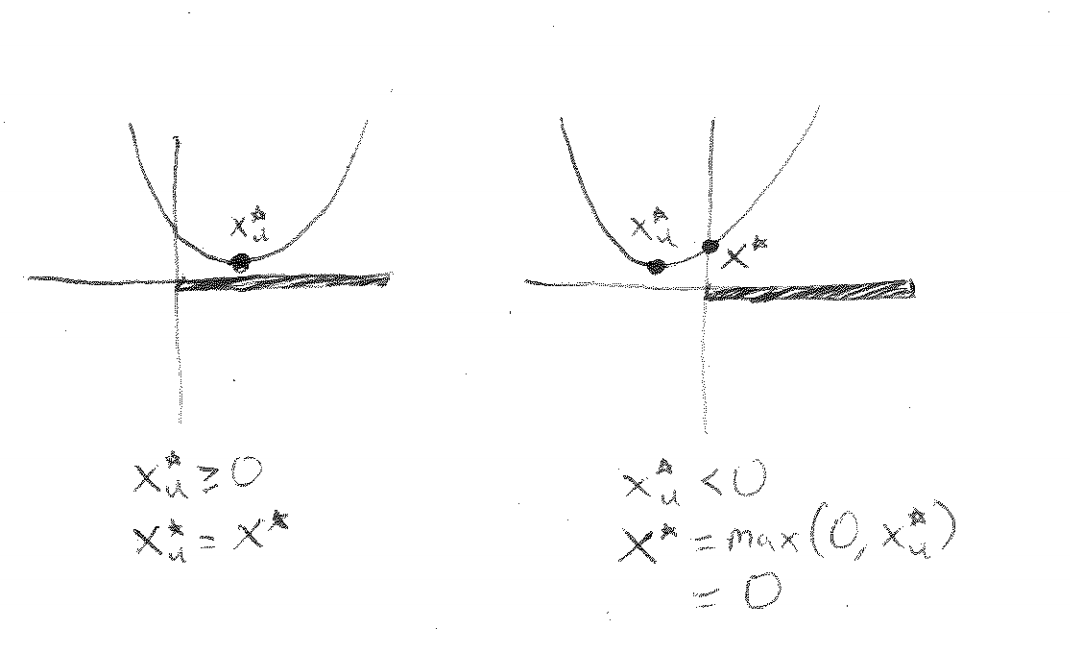
\includegraphics[width=0.5\linewidth]{images/constrained_quadratic.png}
\caption{Optimizing a quadratic function with the constraint $x \geq 0$. The shaded part of the real line represents the feasible set. $x_u^*$ is the global solution to the unconstrained problem. $x^*$ solves the constrained problem.}
\label{conquad}
\end{figure}
%
To see this, consider the unconstrained solution ($x_u^* = b/a$). If $b/a \geq 0$, then the unconstrained solution---which is a global optimizer of the objective over all reals---optimizes the objective of the subset of reals, $x \geq 0$, and we have $x^* = x_u^*$. If $b/a < 0$, then the unconstrained optimum is to the left of 0. The function is \textit{always non-decreasing} to the right of the minimum. Thus, the leftmost point in $\{x \geq 0\}$ must be optimal---$x^*=0$ in ths case. (See the ``proof by picture'' in Figure \ref{conquad} if you don't believe me.)


\item Vector variable ($x \in \Real{n}$), linear objective, linear constraint:
%
\begin{equation*}
p^* = \left\{
\begin{aligned}
\min_{x} \; &a^T x \\
\text{s.t. } \;  &b^T x \geq c 
\end{aligned}
\right\}
= \left\{ \begin{array}{ll}
c \|a\|_2 / \|b\|_2 & a = \gamma b, \text{for } \gamma > 0 \\
-\infty & \text{otherwise}
\end{array}\right.
\end{equation*}
%
Proof: Express $x$ as a sum of two terms, one proportional to $b$, and one perpendicular to $b$ (which we are allowed to do by fundamental theorem of linear algebra---think about it!). Notate this as $x = \alpha b + \nu$, with $\nu^T b = 0$. The problem then becomes:
%
\begin{align*}
p^* &= \min_x a^T x \; : b^T x \geq c \\
&= \min_{\alpha, \nu} a^T (\alpha b + \nu) \; : b^T (\alpha b + \nu) \geq c, \;\;\; \nu^T b = 0  \\
&= \min_{\alpha, \nu} \alpha (a^T b)  + a^T \nu \; : \alpha b^T b \geq c, \;\;\; \nu^T b = 0  \\
&= \min_{\alpha \geq c/ b^T b} \alpha (a^T b) + \min_{\nu : \nu^T b = 0} a^T \nu 
\end{align*}
%
The first problem, minimizing over $\alpha$, gives optimal value $-\infty$ if $a^T b < 0$; if $a^T b > 0$, its optimal point is $\alpha = c / b^T b$ and its optimal value is $c (a^T b) / (b^T b)$.  

The second problem, minimizing over $\nu$, gives optimal value $-\infty$ if $a \not\propto b$. If $a \propto b$, the optimal value is $0$ by the constraint. 

Thus, to have a finite value, we must have $a \propto b$ and $a^T b > 0$; this is achieved when they are co-linear ($a = \gamma b$ for $\gamma \geq 0$). 

\textbf{How should I be able to see this immediately?} This is a problem where you're minimizing a linear function over a halfspace. If the direction of decrease has any component that points \textit{into} the halfspace, then the objective clearly goes to $-\infty$. So the direction of decrease has to point directly out of the halfspace, and then the function is minimized at any point on the hyperplane. (Getting the actual value of the function is just algebra at this point.) If this is still unclear, try Figure \ref{hs}. 

Even though your geometric intuition should point you in the right direction\footnote{yes this was a pun. sorry not sorry}, you should still explain the optimization approach to the solution. (Rigor is good!)

\begin{figure}
\centering
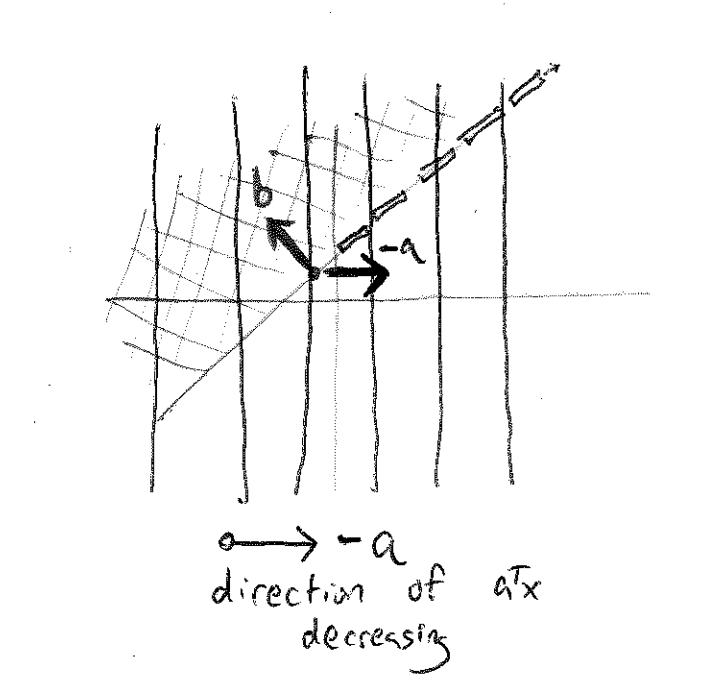
\includegraphics[width=0.5\linewidth]{images/halfspace_optimization.png}
\caption{Optimizing a linear function, $a^T x$, over a halfspace $b^T x \geq c$. The objective decreases in the direction $-a$. If any vector in the hyperplane $b^T x = c$ has positive inner product with $-a$, then the objective decreases as you move along the hyperplane (following the dashed path), and the optimal value is $-\infty$. In order for the optimization problem to have finite value, $a$ must align with $b$.}
\label{hs}
\end{figure}


\item Rayleigh quotient problem: for $A \in \Sym{n}$, 
%
\begin{equation*}
\lambda_{max} (A) = \max_{x} x^T A x \; : \; \|x\|_2 = 1.
\end{equation*}

The proof involves duality, which you haven't learned yet, but you should know this one stone-cold.

\begin{fact} The Rayleigh quotient problem is \textit{nonconvex}, even when $A \succeq 0$.\end{fact} 

The constraint region is the surface of a hypersphere---but does not contain the interior of the hypersphere. (Think about it: is the boundary of a circle a convex set? It has a hole, so it is not.)


\item Relaxed Rayleigh quotient problem: for $A \in \Sym{n}$,
%
\begin{equation*}
\max(0, \lambda_{max} (A)) = \max_x x^T A x \; : \; \|x\|_2 \leq 1.
\end{equation*}

In this problem, we have \textit{relaxed} the constraint, which allows more points in the feasible set. There are two cases here: $\lambda_{max}(A) > 0$, and $\lambda_{max}(A) \leq 0$. In the first case, the optimum value is $\lambda_{max} (A)$ (to see this, compare with the original Rayleigh quotient problem). In the latter case, $A$ is negative-definite, so for any $x \neq 0$, $x^T A x < 0$. Thus, the objective is optimized with $x^* = 0 \implies x^{*T} A x^* = 0$. The $\max(0, \lambda_{max}(A))$ summarizes. 

We could also take a different approach that involves manipulating (reparametrizing) the variables of the optimization problem. Note that
%
\begin{equation*}
\{x \; | \; \|x\|_2 \leq 1\} = \{\alpha z \; | \; \alpha \in [0,1], \; z \in \Real{n}, \; \|z\|_2 = 1\}.
\end{equation*}

This allows us to rewrite the problem as
%
\begin{align*}
\max_{ \|x\|_2 \leq 1 } \; x^T A x \; &= \max_{\begin{subarray}{c} 0 \leq \alpha \leq 1 \\ \|z\|_2 = 1 \end{subarray}} \left( \alpha z \right)^T A (\alpha z) \\
&= \max_{\begin{subarray}{c} 0 \leq \alpha \leq 1 \\ \|z\|_2 = 1 \end{subarray}} \alpha^2 z^T A z \\ 
&= \max_{0 \leq \alpha \leq 1}  \alpha^2 \left( \max_{\|z\|_2 = 1} z^T A z \right) \\
&= \max_{0 \leq \alpha \leq 1}  \alpha^2 \lambda_{max}(A) \\
&= \left\{ \begin{array}{ll}
0 & \lambda_{max}(A) < 0 \\
\lambda_{max}(A) & \text{otherwise}.
\end{array}\right.
\end{align*}

\end{itemize}

\subsection{Equality-Preserving Transformations}

\begin{itemize}
\item \textbf{Epigraph form}: The following is trivially true, for any $R\in\Real{}$:
%
\begin{align*}
R = \min_{t} \;\;& t \\
\text{s.t. } & t \geq R.
\end{align*}

Consequently, we are justified in putting an optimization program in \textit{epigraph form},
%
\begin{align*}
\min_x f(x) = \min_{x,t} \;\;& t \\
\text{s.t. } & t \geq f(x).
\end{align*}

Note that this transformation preserves convexity: if $f$ is a convex function of $f$, the constraint $t \geq f(x)$ is jointly convex in $x$ and $t$. Furthermore, the objective is convex (linear) in the variables of optimization. So, the epigraph form of a convex optimization problem is itself a convex optimization problem.

\item \textbf{Domain-splitting}: For any problem of the form
%
\begin{equation*}
p^* = \min_{x \in \calX} f(x),
\end{equation*}
%
if we can express $\calX = \calY \cup \calZ$ for some sets $\calY, \calZ$, then
%
\begin{equation*}
p^* = \min\left( \min_{x \in \calY} f(x), \; \min_{x \in \calZ} f(z) \right).
\end{equation*}

\item \textbf{Reparametrization}: By fundamental theorem of linear algebra, for any vector $x \in \Real{n}$ and matrix $A \in \Real{n \times m}$, we can write $x = Az + v$ for some $z \in \Real{m}$ and $v \in \calN(A^T)$. So the following optimization problems are equivalent:
%
\begin{align*}
p^* &= \min_{x \in \calX} f(x) \\
&= \min_{z,v} f(Az + v) \; : \; Az + v \in \calX, \; A^T v = 0.
\end{align*} 

\item \textbf{Composing the objective with monotone-increasing functions}: Suppose $\phi : \Real{} \to \Real{}$ is monotone increasing. Then for any $x,y$, $f(x) \geq f(y) \Longleftrightarrow \phi(f(x)) \geq \phi(f(y))$. Thus, the following two problems have the same \textit{optimal sets}:
%
\begin{equation*}
\arg \min_{x \in \calX} f(x) = \arg \min_{x \in \calX} \phi(f(x)),
\end{equation*}
%
and the optimal values are related by
%
\begin{equation*}
\phi\left( \min_{x \in \calX} f(x) \right) = \min_{x \in \calX} \phi(f(x)).
\end{equation*}

\end{itemize}

\subsection{Constraint Magic}

In this section, we deal with common transformations of constraints that you should know about. 

\begin{itemize}
\item \textbf{Max-forall trick}: Suppose you have a constraint of the form
%
\begin{equation}
0 \geq \max_{x \in \calX} f(x). \label{maxconstraint}
\end{equation}

Recall that $\forall y \in \calX, \max_{x \in \calX} f(x) \geq f(y)$. Thus, (\ref{maxconstraint}) \textit{implies} (we're only showing one direction with this step) that
%
\begin{equation}
\forall x \in \calX, \;\; 0 \geq f(x). \label{maxconstraint2}
\end{equation}

Suppose $x^*$ maximizes $f$ in $\calX$. Then (\ref{maxconstraint2}) implies that $0 \geq f(x^*) = \max_{x \in \calX} f(x)$, so the implication goes both ways. We conclude that \textbf{any time you see a constraint on a maximum of a function over a set, you can replace it with multiple constraints, one for each element in the set}:
%
\begin{equation*}
0 \geq \max_{x \in \calX} f(x) \;\;\; \Longleftrightarrow \;\;\; \forall x \in \calX, \;\; 0 \geq f(x).
\end{equation*}

\item \textbf{Absolute value trick}: Suppose you have a constraint of the form
%
\begin{equation*}
|x_i| \leq s_i,
\end{equation*}
% 
for variable $x_i$. This can be rewritten as two inequalities,
%
\begin{equation*}
|x_i| \leq s_i \;\;\; \Longleftrightarrow \;\;\; \begin{array}{c}
x_i \leq s_i, \\
-x_i \leq s_i.
\end{array}
\end{equation*}

The feasible set for $x_i$ is \textbf{convex} in this case: $-s_i \leq x_i \leq s_i$. 

\textbf{CAVEAT: this gets you a convex feasible set (works the way you want it to) when the absolute value of something is bounded ABOVE. If the absolute value is bounded below, you may get a non-convex feasible set. If the constraint is an equality constraint, you definitely get a non-convex feasible set.}

Observe: $|x_i| \geq s_i$ implies $x_i \geq s_i$ or $x_i \leq -s_i$. \textit{This set is not convex for $x_i$ for arbitrary $s_i$.} Similarly, $|x_i| = s_i$ implies $x_i \in \{s_i, -s_i\}$; this set is also not convex for $x_i$. See Figure \ref{absval}.

\begin{figure}
\centering
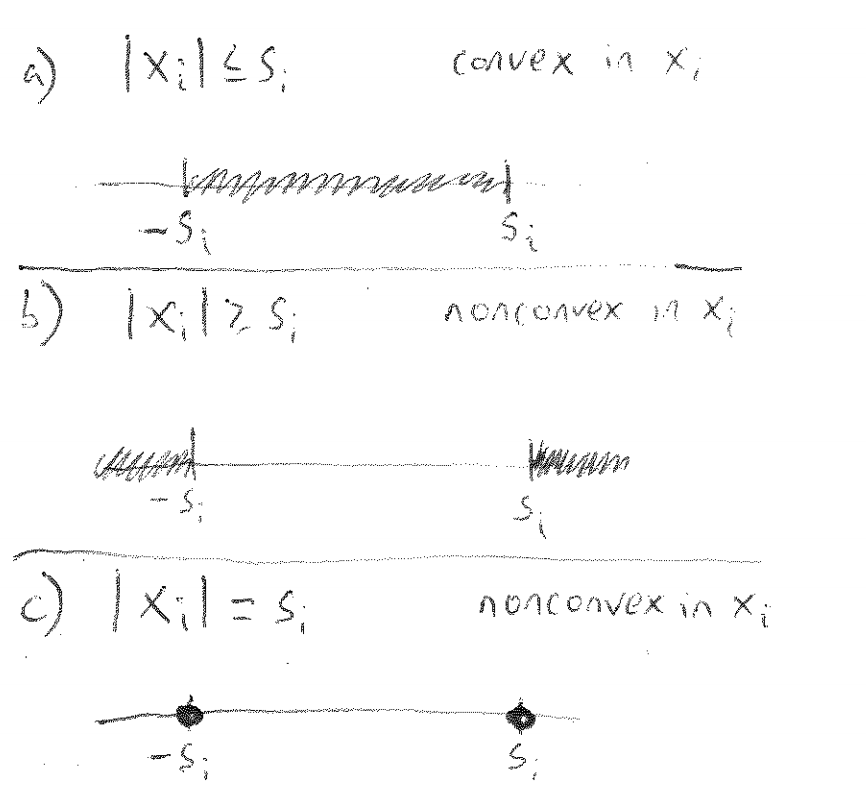
\includegraphics[width=0.5\linewidth]{images/abs_val_trick.png}
\caption{Geometric intuition for constraints involving absolute values. Here, we are considering a case where $s_i \geq 0$.}
\label{absval}
\end{figure}

\end{itemize}

\begin{example} Consider an optimization problem of the form 
%
\begin{equation*}
\min_{x} a^T x + \|x\|_{\infty}.
\end{equation*}
%
We will show that through constraint magic, we can express this problem as an LP. We proceed as follows:
%
\begin{align*}
p^* &= \min_{x} a^T x + \|x\|_{\infty} \\
&= \min_{x,s} a^T x + s \;\; : \;\; s\geq \|x\|_{\infty} && \text{epigraph form of }\|x\|_{\infty}\\
&= \min_{x,s} a^T x + s \;\; : \;\; s\geq \max_i |x_i| && \text{definition of } \|x\|_{\infty}\\
&= \min_{x,s} a^T x + s \;\; : \;\; \forall i, \;\; s\geq |x_i| && \text{max-forall trick}\\
&= \min_{x,s} a^T x + s \;\; : \;\; \forall i, \;\; -s\leq x_i \leq s. && \text{absolute value trick}
\end{align*}
%
In the final step, the objective is linear in $(x,s)$ and the constraints are also linear in $x, s$. (If you have trouble seeing how it's linear in both $x$ and $s$, observe that you can write $\forall i, s - x_i \geq 0, \;\; s + x_i \geq 0$.)


\end{example}


\pagebreak

\section{Duality Intro: Defining Weak and Strong Duality}

In this section, we begin to explore \textbf{duality}, a subject where we study the relationships between the optimization problems
%
\begin{equation*}
\min_{x \in \calX} \max_{y \in \calY} f(x,y),
\end{equation*}
%
which is called a min-max problem, and
%
\begin{equation*}
\max_{y \in \calY} \min_{x \in \calX} f(x,y),
\end{equation*}
%
which is called a max-min problem.

Although the difference may seem subtle, it is crucial: many problems are easier to solve in one formulation than the other, so being able to transform freely between them is highly beneficial. 

Furthermore, the special case of \textbf{Lagrangian duality} allows us to make a wide range of constrained optimization problems analytically solvable.

\subsection{Weak Duality}

\textbf{Proposition.} The principle of \textbf{weak duality} is as follows: for every set $\calX$, set $\calY$, and function $f: \calX \times \calY \to \Real{}$, the following inequality holds:
%
\begin{equation}
p^* \doteq \min_{x \in \calX} \max_{y \in \calY} f(x,y) \geq \max_{y \in \calY} \min_{x \in \calX} f(x,y) \doteq d^*.
\end{equation}

The difference $p^* - d^*$ is called the \textbf{duality gap}. 

\begin{proof}
First, the definitions of optimality give us the following two inequalities:
%
\begin{align*}
\forall x\in \calX, y\in \calY, && \; \max_{\bar{y} \in \calY} f(x, \bar{y}) &\geq f(x,y), \\ 
\forall x\in \calX, y\in \calY, && \; f(x, y) &\geq \min_{\bar{x} \in \calX} f(\bar{x},y).
\end{align*}

It follows immediately that
%
\begin{equation*}
\forall x\in\calX, \forall y \in \calY, \;\;\;\max_{\bar{y} \in \calY} f(x, \bar{y}) \geq \min_{\bar{x} \in \calX} f(\bar{x},y).
\end{equation*}

We use the forall---max equivalence to get:
%
\begin{equation*}
\forall x\in\calX, \;\;\;\max_{\bar{y} \in \calY} f(x, \bar{y}) \geq \max_{y \in \calY} \min_{\bar{x} \in \calX} f(\bar{x},y).
\end{equation*}

Because this holds for all $x$, it holds for the $x$ that minimizes the left-hand side; thus the proof is complete.
\end{proof}

Weak duality \textit{always holds}, and can come in handy sometimes, even though we'll generally prefer strong duality. 

\subsection{Strong Duality}

We say that strong duality holds for a min-max problem when
%
\begin{equation*}
\min_{x \in \calX} \max_{y \in \calY} f(x,y) = \max_{y \in \calY} \min_{x \in \calX} f(x,y).
\end{equation*}

\textbf{Strong duality does not generally hold.} If you want to claim that it does, you have to justify it in some sense. We will talk about the conditions for strong duality to hold later in the notes.

\pagebreak

\section{Duality Intro: Lagrange Dual Problems}

In this section, we deal with \textbf{Lagrange duality}. In Lagrange duality, we study constrained \textbf{primal problems} of the form
%
\begin{equation}
\begin{aligned}
p^* = \min_{x} \;\;& f_0(x) \\
\text{s.t. } \;\;&  f_i (x) \leq 0, \;\;\; i = 1, ..., m \\
& h_i (x) = 0, \;\;\; i= 1, ..., p.
\end{aligned} \label{primal}
\end{equation}

This constrained primal problem is equivalent to the following min-max optimization problem:
%
\begin{equation}
p^* = \min_x \max_{\lambda \succeq 0, \nu} f_0 (x) + \sum_{i=1}^m \lambda_i f_i (x) + \sum_{j=1}^p \nu_j h_j (x). \label{minmax}
\end{equation}
%
Here, we interpret the \textbf{dual variables} $\lambda, \nu$ to be the Lagrange multipliers (which you might remember from calculus). Observe that the optimization over $x$ is now \textit{unconstrained}: the constraints have been added to the objective as penalty terms, where a violation receives an infinite penalty. 

The optimization objective in (\ref{minmax}) has a special name: we call it the Lagrangian, $\calL$, and it is a function of both the primal and dual variables:
%
\begin{equation*}
\calL(x, \lambda, \nu) \doteq f_0 (x) + \sum_{i=1}^m \lambda_i f_i (x) + \sum_{j=1}^p \nu_j h_j (x).
\end{equation*}
%
The act of moving a constraint function into the objective by Lagrange multipliers is called \textit{dualizing} the constraint. 

A lower bound on $p^*$ can be found by switching the min and the max:
%
\begin{equation}
p^* \geq d^* \doteq \max_{\lambda \succeq 0, \nu} \min_x  f_0 (x) + \sum_{i=1}^m \lambda_i f_i (x) + \sum_{j=1}^p \nu_j h_j (x). \label{maxmin}
\end{equation}
%
That this is a lower bound follows from the principle of weak duality.

The function which is obtained by solving the inner optimization problem over $x$, for fixed $\lambda, \nu$, is called the \textbf{Lagrange dual function}, and it is usually denoted by $g(\lambda, \nu)$:
%
\begin{equation*}
g(\lambda, \nu) \doteq \min_x f_0 (x)+ \sum_{i=1}^m \lambda_i f_i (x) + \sum_{j=1}^p \nu_j h_j (x).
\end{equation*}

The problem of optimizing the Lagrange dual function over the dual variables is called a \textbf{Lagrange dual problem}, or simply the dual problem:
%
\begin{equation*}
d^* = \max_{\lambda \succeq 0, \nu} g(\lambda, \nu).
\end{equation*}

\subsection{Why Does the Min-Max Formulation Work?}

In this section, we aim to verify that the primal problem shown in (\ref{primal}) is equivalent to the min-max problem shown in (\ref{minmax}). 

We will begin from the min-max form (\ref{minmax}), and solve the inner maximization problems over $\lambda, \nu$.

We proceed by first exploiting the fact that the optimization over $\lambda, \nu$ is \textit{decoupled}:
%
\begin{align*}
& \min_x \max_{\lambda \succeq 0, \nu} f_0 (x) + \sum_{i=1}^m \lambda_i f_i (x) + \sum_{j=1}^p \nu_j h_j (x) \\
&= \min_x \left( f_0 (x) + \sum_{i=1}^m \left(\max_{\lambda_i \geq 0} \lambda_i f_i (x)\right) + \sum_{j=1}^p \left( \max_{\nu} \nu_j h_j (x) \right) \right).
\end{align*}

Now, let's examine the sub-problems over the $\lambda$'s and the $\nu$'s. \textbf{Notice that the optimization over $\lambda$ is constrained to $\lambda \succeq 0$, but no such constraint exists over $\nu$. This is important.}

\textbf{The sub-problem over $\lambda_i$:}
%
\begin{equation*}
\max_{\lambda_i \geq 0} \; \lambda_i f_i (x) = \left\{ \begin{array}{ll}
0 & f_i (x) \leq 0 \\
\infty & f_i (x) > 0.
\end{array} \right.
\end{equation*}

\textbf{The sub-problem over $\nu_j$:}
%
\begin{equation*}
\max_{\nu_j \geq 0} \; \nu_j h_j(x) = \left\{ \begin{array}{ll}
0 & h_j (x) = 0 \\
\infty & h_j (x) \neq 0.
\end{array} \right.
\end{equation*}

Adding up the contributions from all the different terms, we get
%
\begin{align*}
& \min_x \left( f_0 (x) + \sum_{i=1}^m \left(\max_{\lambda_i \geq 0} \lambda_i f_i (x)\right) + \sum_{j=1}^p \left( \max_{\nu} \nu_j h_j (x) \right) \right) \\
&= \min_x \left\{ \begin{array}{ll} 
f_0 (x)  & \text{if } f_i (x) \leq 0, \text{for } i=1, ..., m, \;\;\; h_j (x) = 0, \text{for } j = 1, ..., p, \\
\infty & \text{otherwise}.
\end{array} \right.
\end{align*}

Suppose that there is any point $x$ which satisfies $f_i (x) \leq 0$ for all $i$ and $h_j (x) = 0$ for all $j$, and for which $f_0 (x)$ is well-defined (takes a finite value). Then that point is strictly better than any point which does not satisfy all of those constraints (because in those cases, the penalized objective has value infinity). Thus we can remove those points from the feasible set without changing the optimal point or value: that is, 
%
\begin{align*}
& \min_x \left\{ \begin{array}{ll} 
f_0 (x)  & \text{if } f_i (x) \leq 0, \text{for } i=1, ..., m, \;\;\; h_j (x) = 0, \text{for } j = 1, ..., p, \\
\infty & \text{otherwise}.
\end{array} \right. \\
&= \min_x f(x) \;\; : \;\; f_i (x) \leq 0 \;\; \text{for } i=1,..., m, \;\; h_j (x) = 0 \;\; \text{for } j=1,..., p. 
\end{align*}

Intuitively, \textbf{if you replace constraints with penalty functions in the objective, and you make the penalty infinitely steep for violating the constraint, your penalized formulation is equivalent to your constrained formulation}. 


\subsection{Lagrange Dual Problems Always Exist}

Regardless of whether or not strong duality holds (that is, regardless of whether or not $p^* = d^*$), \textbf{we can always form a Lagrange dual problem}. 

\subsection{Lagrange Dual Problems Are Not Unique}

There can be many equivalent ways to express the same set of constraints, resulting in many different Lagrange dual problems for the same primal problem. Some of these formulations are more useful than others. 

For example, let's study a very simple case where things quickly go \textit{horribly wrong} if we make a bad choice of how to represent and dualize the constraints.

\begin{example}
The primal problem under consideration is
%
\begin{equation}
p^* = \min_x\; \frac{1}{2} \|x\|_2^2 + b^T x \;\;\; : \;\;\;  (c^T x)^2 \leq 1. 
\end{equation}

\textbf{Dualizing the Constraint As-Is}:

The constraint is simple-looking, so dualizing it shouldn't be too hard. What happens when we try to dualize it, as-is, and find a dual problem?

We proceed:
%
\begin{align*}
p^* &= \min_x \;\frac{1}{2} \|x\|_2^2 + b^T x \;\;\; : \;\;\;  (c^T x)^2 \leq 1 \\
&= \min_x \max_{\lambda \geq 0} \; \frac{1}{2} \|x\|_2^2 + b^T x + \frac{1}{2} \lambda \left( (c^T x)^2 - 1 \right) \\
&\geq \max_{\lambda \geq 0} \min_x  \; \frac{1}{2} \|x\|_2^2 + b^T x + \frac{1}{2} \lambda \left( (c^T x)^2 - 1 \right) \\
&\doteq d^*.
\end{align*}

At this stage, we rewrite the objective, with $\|x\|_2^2 = x^T x$ and $(c^T x)^2 = x^T (c c^T ) x$, and try to solve for the dual function
%
\begin{equation*}
g(\lambda) = \min_x \; \calL(x,\lambda), \;\;\; \text{where } \calL(x,\lambda) \doteq \frac{1}{2} x^T \left( I + \lambda c c ^T \right) x + b^T x - \lambda.
\end{equation*}
%
Note that this is \textit{unconstrained, convex, quadratic} optimization, which is easy---set the gradient to zero and solve. We find:
%
\begin{equation*}
\nabla_x \calL(x,\lambda) = (I + \lambda c c ^T) x^* + b = 0 \;\;\; \Longrightarrow \;\;\; x^* (\lambda) = - (I + \lambda c c^T)^{-1} b.
\end{equation*}

After plugging this $x^* (\lambda)$ back in, we obtain the dual function
%
\begin{equation*}
g(\lambda) = - \frac{1}{2} b^T (I + \lambda c c^T)^{-1} b - \lambda,
\end{equation*}
%
and the corresponding dual problem,
%
\begin{equation*}
d^* = \max_{\lambda \geq 0} - \frac{1}{2} b^T (I + \lambda c c^T)^{-1} b - \lambda.
\end{equation*}

This is a horrible, awful dual problem that is functionally useless to us. Observe how $\lambda$ appears in it: it shows up inside a matrix inverse. This is a super complicated dependence that makes things almost totally analytically intractable. Bad. Avoid this.


\textbf{Dualizing Equivalent Constraints Instead}:

Observe that $(c^T x)^2 \leq 1$ is equivalent to $-1 \leq c^T x \leq 1$. Instead of dualizing the original quadratic constraint, let's dualize the equivalent linear constraints and see what happens.

The problem becomes:
%
\begin{align*}
p^* &= \min_x \;\frac{1}{2} \|x\|_2^2 + b^T x \;\;\; : \;\;\;  -1 \leq c^T x \leq 1 \\
&= \min_x \max_{\lambda_1, \lambda_2 \geq 0} \; \frac{1}{2} \|x\|_2^2 + b^T x + \lambda_1 \left(c^T x - 1 \right) + \lambda_2 \left(-1 - c^T x \right) \\
&\geq \max_{\lambda_1, \lambda_2 \geq 0} \min_x \; \frac{1}{2} \|x\|_2^2 + b^T x + \lambda_1 \left(c^T x - 1 \right) + \lambda_2 \left(-1 - c^T x \right) \\
&\doteq d^*.
\end{align*}

We obtain the dual function the same way as before---by solving the inner optimization over $x$, by setting the gradient (wrt $x$) of the Lagrangian equal to zero and solving:
%
\begin{equation*}
\nabla_x \calL(x,\lambda_1, \lambda_2) = x^* + b + \lambda_1 c - \lambda_2 c = 0 \;\;\; \Longrightarrow \;\;\; x^* (\lambda_1, \lambda_2) = -b - \lambda_1 c + \lambda_2 c.
\end{equation*}

After plugging this $x^*(\lambda_1, \lambda_2)$ back in, we obtain the dual function:
%
\begin{align*}
g(\lambda) &\doteq -\frac{1}{2} \left(b +\lambda_1 c - \lambda_2 c\right)^T (b + \lambda_1 c - \lambda_2 c) - \lambda_1 - \lambda_2,
\end{align*}
%
which we can see is \textit{quadratic} in $\lambda_1, \lambda_2$ - this is much nicer than before. 

\end{example}

\subsection{Lagrange Dual Problems for Maximization Primal Problems}

Sometimes, the primal problem is a maximization problem and not a minimization problem. This poses no issue to forming a Lagrange dual---which will in this case turn out to be a minimization over the dual variables rather than a maximization---but we do have to be careful about signs.

The way we dualize constraints in this case is as follows:
%
\begin{align*}
& \max_x f_0(x) \;\; : \;\; f_i (x) \leq 0 \;\; \text{for } i=1,..., m, \;\; h_j (x) = 0 \;\; \text{for } j=1,..., p. \\
&= \max_x \min_{\lambda \geq 0, \nu} f_0(x) - \sum_{i=1}^m \lambda_i f_i(x) + \sum_{j=1}^p \nu_j h_j (x).
\end{align*}

\textbf{Note that we have a minus sign in front of $\lambda_i$ now, unlike before. This is important.}

\textbf{Minor exercise.} Verify that this max-min problem is equivalent to the original max problem by showing that the inner minimization problem has the solution
%
\begin{equation*}
\left\{\begin{array}{ll}
f_0 (x) & \text{if } f_i (x) \leq 0 \text{ for } i=1,..., m, \;\; h_j(x) = 0 \text{ for } j=1,..., p, \\
-\infty & \text{otherwise}.
\end{array}\right.
\end{equation*}

The dual function in this case is
%
\begin{equation*}
g(\lambda, \nu) = \max_x f_0(x) - \sum_{i=1}^m \lambda_i f_i(x) + \sum_{j=1}^p \nu_j h_j (x),
\end{equation*}
%
and the dual problem is
%
\begin{equation*}
\min_{\lambda \succeq 0, \nu} g(\lambda, \nu).
\end{equation*}

\pagebreak

\section{Duality Intro: When Does Strong Duality Hold?}


In this section, we will give two theorems for when strong duality holds. These are Slater's theorem, which gives a simple condition for strong duality of Lagrange dual problems, and Sion's minimax theorem, which gives very general conditions under which strong duality is attained. 

Because these theorems concern min-max problems, they are called \textbf{minimax theorems}.  

\subsection{Strong Duality for Lagrange Dual Problems}

\begin{theorem}[Slater's Theorem] 
Suppose the primal problem, 
%
\begin{equation*}
\begin{aligned}
p^* = \min_{x} \;\;& f_0(x) \\
\text{s.t. } \;\;&  f_i (x) \leq 0, \;\;\; i = 1, ..., m \\
& h_i (x) = 0, \;\;\; i= 1, ..., p.
\end{aligned}
\end{equation*} 
%
is a convex optimization problem. Let $\calD$ denote the domain of the problem, $\calD \doteq \dom(f) \cap \bigcap_{i=1}^m \dom(f_i)  \cap \bigcap_{i=1}^n \dom(h_i)$. Suppose that there exists an $x \in \relint{\calD}$ such that
%
\begin{equation*}
f_i(x) < 0, \;\; i=1,...,m, \;\;\; h_i (x) = 0, \;\; i=1,...,n.
\end{equation*}
%
Then strong duality holds, in that, for the Lagrangian
%
\begin{equation*}
\calL(x,\lambda, \nu) = f(x) + \sum_{i=1}^m \lambda_i f_i (x) + \sum_{i=1}^n \nu_i h_i (x),
\end{equation*}
%
we have
%
\begin{equation*}
p^* = \min_x \max_{\lambda \geq 0, \nu} \calL(x,\lambda, \nu) = \max_{\lambda \geq 0, \nu} \min_x  \calL(x,\lambda, \nu)  = d^*.
\end{equation*}

A weaker form of this holds if the first $k$ inequality constraints are affine: then there only needs to exist an $x \in \relint{\calD}$ such that
%
\begin{equation*}
f_i(x) \leq 0, \;\; i=1,...,k, \;\;\; f_i(x) < 0, \;\; i=k+1,...,m, \;\;\; h_i (x) = 0, \;\; i=1,...,n.
\end{equation*}
%
for strong duality to hold.
\end{theorem}

Note that \textbf{Slater's theorem only works for Lagrangians that you build by dualizing constraints}. This cannot be applied to arbitrary min-max problems: you need to have the primal constrained problem to make this work. 

\subsection{Strong Duality for General Min-Max Problems}

\begin{theorem}[Sion's Minimax Theorem] 
For a function $\calL : X \times Y \to \Real{}$, if $X$ is a compact and convex subset of a linear topological space and $Y$ is a convex subset of a linear topological space, and
%
\begin{itemize}
	\item $\forall x \in X$, $\calL(x,\cdot)$ is quasiconcave and upper semi-continuous, and 
	\item $\forall y \in Y$, $\calL(\cdot,y)$ is quasiconvex and lower semi-continuous, 
\end{itemize}
%
then
%
\begin{equation*}
\min_{x \in X} \sup_{y \in Y} \calL(x,y) = \sup_{y\in Y} \min_{x\in X} \calL(x,y).
\end{equation*}
\end{theorem}

Notes on Sion's theorem:
%
\begin{itemize}
\item Don't worry about what a linear topological space is. $\Real{n}$ (with a normal dot product) is a linear topological space and that is the only one you need to care about. 
\item Quasiconcavity and quasiconvexity are sort-of generalizations of concavity and convexity. All concave functions are quasiconcave (but not vice-versa), and all convex functions are quasiconvex (but not vice-versa).
\item If something is continuous it is also both upper and lower semi-continuous. 
\item A compact set contains its limit points. The open interval $(a, b) \subset \Real{}$ is not compact. The closed interval $[a,b] \subset \Real{}$ is compact. The set $\{x \; : \; \|x\|_p \leq 1\}$ is compact.
\item You have to satisfy conditions on both the Lagrangian function $\calL$, and the feasible sets $X, Y$ in order to apply Sion's theorem.
\end{itemize}

If you see a Lagrangian function $\calL(x,y)$ that is concave in $y$, convex in $x$, and continuous, it satisfies the conditions of Sion's theorem for the Lagrangian. 

If both feasible sets $X$ and $Y$ are convex, and at least one of them is compact, that's sufficient for Sion's theorem. 

We have experienced some difficulty with the compactness condition in some problems---if this is an issue in your homework and you can't prove strong duality any other way, don't worry about this hiccup. There is probably some other theorem that can save you. 

\pagebreak

\section{KKT Conditions}


The Karush-Kuhn-Tucker (KKT) conditions characterize optimality for primal problem / Lagrange dual problem pairs when all functions involved are differentiable with respect to $x$. \textbf{These only work for problems that have the Lagrange duality structure. Not for arbitrary min-max problems.} 

Let $x^*$ and $(\lambda^*, \nu^*)$ be any primal and dual optimal points with zero duality gap (that is, $p^* = d^*$). Any such points must satisfy
%
\begin{eqnarray*}
0 &\geq& f_i (x^*) \;\;\; i=1,...,m\\
0&=& h_i (x^*) \;\;\; i=1,...,n \\
0 & \preceq & \lambda^* \\
0 &=& \lambda_i^* f_i (x^*) \;\;\; i=1,...,m \\
0 &=& \nabla_x f_0 (x^*) + \sum_{i=1}^m \lambda_i^* \nabla f_i(x^*) + \sum_{i=1}^n \nu_i^* \nabla h_i (x^*).
\end{eqnarray*}

When the primal problem is convex, the KKT conditions are also sufficient conditions for the primal and dual points to be optimal: if $x^*$ and $(\lambda^*, \nu^*)$ are any points that satisfy the KKT conditions, then they are primal and dual optimal for that problem.

Notes on the KKT conditions: 
%
\begin{itemize}
\item The first three conditions just require $x^*, \lambda^*$ to be primal and dual feasible, respectively.
\item The last condition comes from solving the unconstrained minimization problem over $x$: to compute $
\min_x \calL(x,\lambda^*,\nu^*)$, we set the gradient to zero:
%
\begin{equation*}
\nabla_x \calL (x^*, \lambda^*, \nu^*) = \nabla_x f_0 (x^*) + \sum_{i=1}^m \lambda_i^* \nabla f_i(x^*) + \sum_{i=1}^n \nu_i^* \nabla h_i (x^*) = 0.
\end{equation*}
\item The fourth condition, $\lambda_i^* f_i (x^*) = 0$, is called \textbf{complementary slackness}. This is an interesting and subtle condition, but proving it is straightforward. Suppose $f_i (x^*) < 0$. What is 
%
\begin{equation*}
\lambda_i^* = \arg \max_{\lambda_i \geq 0} \; \lambda_i f_i (x^*)?
\end{equation*}
%
Spoiler alert: $\lambda_i^* = 0$. Thus, for this case, $\lambda_i^* f_i (x^*) = 0$. What about in the case where $f_i (x^*) = 0?$ This case seems to solve itself. The case $f_i (x^*) > 0$ is not possible (it violates a feasibility condition for $x^*$), so we don't have to worry about it. 

\end{itemize}


\pagebreak

\section{\href{http://catb.org/jargon/html/magic-story.html}{More Magic}}

In this section, I'll go through a few magic tricks that don't specifically fit anywhere else, but are neat and will add to your understanding / problem-solving ability:
%
\begin{itemize}
\item the norm trick,
\item the $\min \Leftrightarrow \exists$ trick,
\item and the business of when to turn a bad case of the infinities into a constraint. 
\end{itemize}

\subsection{The Norm Trick}

Calling this a trick is maybe somewhat misleading. So first, let's get on solid ground. Given a norm $\|\cdot \|$, we define the dual norm $\|\cdot\|_*$ by:
%
\begin{equation*}
\|x\|_* \doteq \max_{z} z^T x \; : \; \|z\| \leq 1.
\end{equation*}

The ``trick'' is that the $p$-norm and the $q$-norm, for $1/p + 1/q = 1$, are dual norms to each other: that is,
%
\begin{equation*}
\|x\|_p = \max_z z^T x \;\; : \;\; \|z\|_q \leq 1,
\end{equation*}
%
where $1/p + 1/q = 1$, and $\| \cdot \|_p$ is the $l_p$-norm, defined by $\|z\|_p = (\sum_i z_i^p)^{1/p}$. 


\begin{example}
Consider the problem 
%
\begin{equation}
p^* = \min_{x \in X} f(x) + \lambda \|x\|_2.
\label{exconv}
\end{equation}

The norm ``trick'' allows us to rewrite the $l_2$-norm regularization in (\ref{exconv}) as
%
\begin{equation*}
p^* = \min_{x \in X} \max_{z} f(x) + \lambda z^T x \;\; : \;\; \|z\|_2 \leq 1.
\end{equation*}
%
If $f$ is convex and $X$ is a convex subset of $\Real{n}$, Sion's theorem tells us that strong duality holds. (Note that we have compactness on the $z$-set.) 
\end{example}

\subsection{``Min---There Exists'' Trick}

In the special review session, a robust-constraint problem came up with the form
%
\begin{equation*}
\min_{x \in \calX} f(x) \; : \; \left(\min_{z \in \calZ} z^T x\right) \leq b.
\end{equation*}

The interesting thing is that this problem is equivalent to
%
\begin{equation*}
\min_{x \in \calX, z \in \calZ} f(x) \; : \; z^T x \leq b.
\end{equation*}

In this latter form, we've lifted up the variable $z$ from only existing in a sub-problem in the constraint, to being a variable in the overall optimization. How did we do this?

It's conceptually similar to the $\max$---forall trick. The equivalence is this:
%
\begin{equation*}
\left(\min_{z \in \calZ} z^T x \right) \leq b\;\;\; \Longleftrightarrow \exists z \in \calZ \; : \; z^T x \leq b.
\end{equation*}

Proving this is straightforward. First, consider the forward direction. If $\left(\min_{z \in \calZ} z^T x \right) \leq b$, then there is some $z$ (perhaps the minimizer) such that $z^T x \leq b$. 

Consider the reverse direction. Suppose there is some $\bar{z} \in \calZ $ such that $\bar{z}^T x \leq b$. We know that by definition, $\min_{z \in \calZ} z^T x \leq \bar{z}^T x$, so it follows transitively that $\min_{z \in \calZ} z^T x \leq b$. QED. 

Note that \textbf{if a variable in an optimization problem does not appear in the objective, but does appear in a constraint, then solving for that variable is simply a feasibility problem.}


\subsection{Bad Case of the Infinities}

The following statements are always true as long as $\calX$ is not empty and $f(x)$ is well-defined everywhere on $\calX$:
%
\begin{align*}
&\min_x \left\{ \begin{array}{ll}
f(x) & x \in \calX \\
\infty & \text{otherwise}
\end{array} \right.\\
&= \min_x \; f(x) \;\;\; : \;\;\; x \in \calX,
\end{align*}  
%
and
%
\begin{align*}
&\max_x \left\{ \begin{array}{ll}
f(x) & x \in \calX \\
-\infty & \text{otherwise}
\end{array} \right.\\
&= \max_x \; f(x) \;\;\; : \;\;\; x \in \calX.
\end{align*}  


That is, if you are optimizing a function with multiple cases, and one of the cases drives the function to the wrong end of infinity ($+\infty$ if you are minimizing, and $-\infty$ if you are maximizing), then you can turn the unconstrained optimization problem into an equivalent constrained problem by turning the condition into a constraint. 

\end{document}

